\documentclass[14pt,a4paper]{scrartcl}
\usepackage[utf8]{inputenc}
\usepackage{ragged2e}
\usepackage{epigraph}
\usepackage{graphicx}
% \usepackage{esint}
\usepackage[english,russian, ukrainian]{babel}
\usepackage{misccorr,color,ragged2e,amsfonts,amsthm,graphicx,systeme,amsmath,mdframed,lipsum}
\usepackage{mathtools}
\renewcommand\qedsymbol{$\blacksquare$}
\renewcommand*{\proofname}{\text{Доведення}}
\theoremstyle{definition}
\newtheorem*{defo}{Означення}
\newtheorem*{teo}{Теорема}
\newtheorem*{example}{Приклад}
\theoremstyle{remark}
\newtheorem*{remark}{Зауваження}
\theoremstyle{definition}
\newtheorem*{consequence}{Наслідок}
\theoremstyle{definition}
\newtheorem{statement}{Утверждение}[section]
\newmdtheoremenv{boxteo}{Теорема}[section]
\setlength\parindent{0pt}
\DeclareMathOperator*\lowlim{\underline{lim}}
\DeclareMathOperator*\uplim{\overline{lim}}
\newcommand\independent{\protect\mathpalette{\protect\independenT}{\perp}}
\def\independenT#1#2{\mathrel{\rlap{$#1#2$}\mkern2mu{#1#2}}}
%
% \makeatletter
% %% make esint definition in line with amsmath
% \@for\next:={int,iint,iiint,iiiint,dotsint,oint,oiint,sqint,sqiint,
%   ointctrclockwise,ointclockwise,varointclockwise,varointctrclockwise,
%   fint,varoiint,landupint,landdownint}\do{%
%     \expandafter\edef\csname\next\endcsname{%
%       \noexpand\DOTSI
%       \expandafter\noexpand\csname\next op\endcsname
%       \noexpand\ilimits@
%     }%
%   }
% \makeatother
% Default fixed font does not support bold face
\DeclareFixedFont{\ttb}{T1}{txtt}{bx}{n}{12} % for bold
\DeclareFixedFont{\ttm}{T1}{txtt}{m}{n}{12}  % for normal

% !!!!!!!!!!!!!!! HEART


% Custom colors
\usepackage{color}
\definecolor{deepblue}{rgb}{0,0,0.5}
\definecolor{deepred}{rgb}{0.6,0,0}
\definecolor{deepgreen}{rgb}{0,0.5,0}

\usepackage{listings}

% Python style for highlighting
\newcommand\pythonstyle{\lstset{
language=Python,
basicstyle=\ttm,
otherkeywords={self},             % Add keywords here
keywordstyle=\ttb\color{deepblue},
emph={MyClass,__init__},          % Custom highlighting
emphstyle=\ttb\color{deepred},    % Custom highlighting style
stringstyle=\color{deepgreen},
frame=tb,                         % Any extra options here
showstringspaces=false            %
}}

\definecolor{javared}{rgb}{0.6,0,0} % for strings
\definecolor{javagreen}{rgb}{0.25,0.5,0.35} % comments
\definecolor{javapurple}{rgb}{0.5,0,0.35} % keywords
\definecolor{javadocblue}{rgb}{0.25,0.35,0.75} % javadoc

\lstset{language=C++,
basicstyle=\ttfamily,
keywordstyle=\color{javapurple}\bfseries,
stringstyle=\color{javared},
commentstyle=\color{javagreen},
morecomment=[s][\color{javadocblue}]{/**}{*/},
numbers=left,
numberstyle=\tiny\color{black},
stepnumber=2,
numbersep=10pt,
tabsize=4,
showspaces=false,
showstringspaces=false}


% Python environment
\lstnewenvironment{python}[1][]
{
\pythonstyle
\lstset{#1}
}
{}

% Python for external files
\newcommand\pythonexternal[2][]{{
\pythonstyle
\lstinputlisting[#1]{#2}}}

% Python for inline
\newcommand\pythoninline[1]{{\pythonstyle\lstinline!#1!}}
%
% \begin{python}
% class MyClass(Yourclass):
%     def __init__(self, my, yours):
%         bla = '5 1 2 3 4'
%         print bla
% \end{python}

\begin{document}



\def\be{\begin{equation}}
\def\ee{\end{equation}}
\def\bd{\begin{defo}}
\def\ed{\end{defo}}
\def\bbt{\begin{boxteo}}
\def\ebt{\end{boxteo}}
\def\i{\infty}
\def\d{\partial}


\begin{titlepage}
\centering
	\vspace{1cm}
	{ МІНІСТЕРСТВО ОСВІТИ І НАУКИ УКРАЇНИ\\
  НАВЧАЛЬНО-НАУКОВИЙ КОМПЛЕКС\\
  ``ІНСТИТУТ ПРИКЛАДНОГО СИСТЕМНОГО АНАЛІЗУ``\\
  НАЦІОНАЛЬНОГО ТЕХНІЧНОГО УНІВЕРСИТЕТУ УКРАЇНИ\\
  ``КИЇВСЬКИЙ ПОЛІТЕХНІЧНИЙ ІНСТИТУТ ІМЕНІ ІГОРЯ СІКОРСЬКОГО``\\
  КАФЕДРА МАТЕМАТИЧНИХ МЕТОДІВ  СИСТЕМНОГО АНАЛІЗУ\\\par}
	\vspace{5cm}
	{\large Розрахункова робота \\
\textbf{ВИПАДКОВІ ВЕКТОРИ\\ Варіант-93(27)} \\ \par}
	\vfill
  \begin{flushright}
  Виконав:\\
   Терещенко Денис, КА-96\\

  \end{flushright}


	\vfill

% Bottom of the page
	{\large КИЇВ - 2020 \par}
\end{titlepage}
\begin{center} 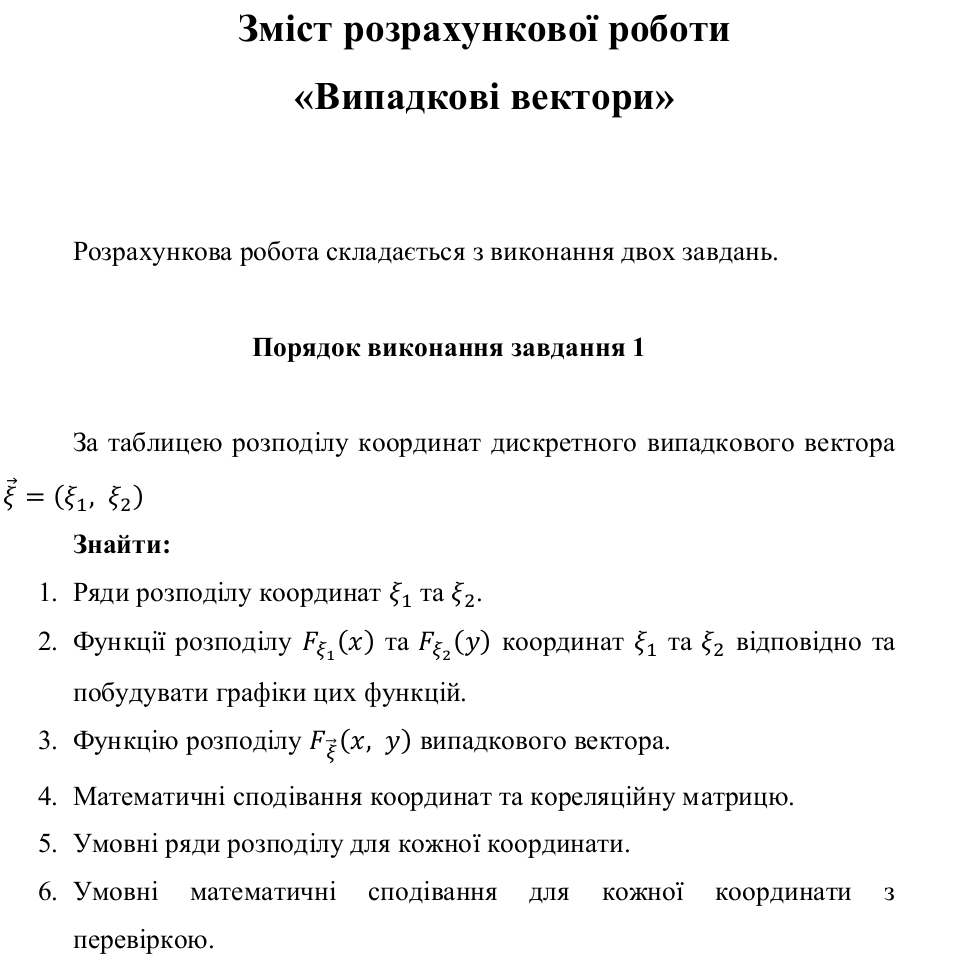
\includegraphics[scale=0.5]{assets/1.png} \end{center}
\begin{center} 
\includegraphics[scale=0.5]{assets/2.png} \end{center}
\begin{center} 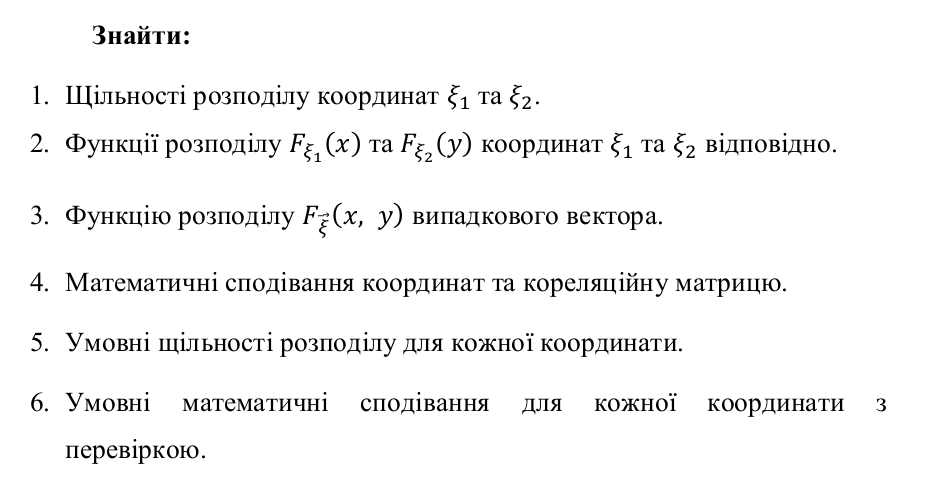
\includegraphics[scale=0.5]{assets/3.png} \end{center}
\tableofcontents

\newpage

\section{Завдання 1}
Дискретний випадковий вектор $\xi = \begin{bmatrix}
 \xi_1 & \xi_2
\end{bmatrix}$ задано таблицею розподілу.

\begin{center}
 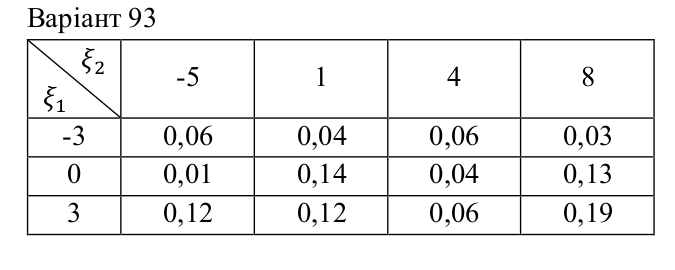
\includegraphics[scale=0.5]{assets/z193.png}\\
Таблиця розподілу згідно варіанту.
  \end{center}
Позначимо ймовірності: $ p_{ij} = \mathbb{P} \left\lbrace \xi_1 = x_i, \xi_2 = y_j \right\rbrace, i = \overline{1,3}, j = \overline{1,4}$
\subsection{Ряди розподілу координат $\xi_1$ та $\xi_2$}
Т.я. події $\left\lbrace \xi_1 = x_i \right\rbrace, i = \overline{1,3}$ утворюють повну группу подій, (як і $\left\lbrace \xi_2 = y_j \right\rbrace, \\j=\overline{1,4} $), можемо скористатися формулою повної ймовірності:\\
$$\mathbb{P} \left\lbrace \xi_1  = x_i \right\rbrace =  \sum\limits_{j = 1}^{ 4}{ p_{ij}} \qquad \mathbb{P} \left\lbrace \xi_2 = y_j \right\rbrace =  \sum\limits_{i = 1}^{ 3}{ p_{ij}}$$

Отримали:
$$\mathbb{P} \left\lbrace \xi_1 =  -3  \right\rbrace =  0.06 + 0.04 + 0.06 + 0.03 = 0.19 $$
$$\mathbb{P} \left\lbrace \xi_1 =  0  \right\rbrace =  0.01 + 0.14 + 0.04 + 0.13 = 0.32 $$
$$\mathbb{P} \left\lbrace \xi_1 =  3  \right\rbrace =  0.12 + 0.12 + 0.06 + 0.19 = 0.49 $$
Перевірка: $ \sum\limits_{i = 1}^{ 3}{ \mathbb{P}\left\lbrace \xi_1 = x_i \right\rbrace} =  0.19 + 0.32 + 0.49  =  1.0 $\\
Отримали:
$$\mathbb{P} \left\lbrace \xi_2 =  -5  \right\rbrace =  0.06 + 0.01 + 0.12 = 0.19 $$
$$\mathbb{P} \left\lbrace \xi_2 =  1  \right\rbrace =  0.04 + 0.14 + 0.12 = 0.3 $$
$$\mathbb{P} \left\lbrace \xi_2 =  4  \right\rbrace =  0.06 + 0.04 + 0.06 = 0.16 $$
$$\mathbb{P} \left\lbrace \xi_2 =  8  \right\rbrace =  0.03 + 0.13 + 0.19 = 0.35 $$
Перевірка: $ \sum\limits_{j = 1}^{4}{ \mathbb{P}\left\lbrace \xi_2 = y_j \right\rbrace} =  0.19 + 0.3 + 0.16 + 0.35  =  1.0 $\\
Ряди розподілу $\xi_1$ та $\xi_2$:
\begin{center}
\begin{tabular}{|c|c|c|c|}
\hline
$\xi_1$ & -3 & 0 & 3 \\ \hline
P & 0.19 & 0.32 & 0.49 \\ \hline
\end{tabular} \qquad \qquad
\begin{tabular}{|c|c|c|c|c|}
\hline
$\xi_2$ & -5 & 1 & 4 & 8 \\ \hline
P       & 0.19  & 0.3 & 0.16 & 0.35 \\ \hline
\end{tabular}
\end{center}

\newpage

\subsection{Функції розподілу координат $\xi_1, \xi_2$.}
Для $\xi_1:$
$$F_{\xi_1}(x) = \mathbb{P} \left\lbrace \xi_1 < x \right\rbrace =
\begin{cases}
	\mathbb{P} \left\lbrace \emptyset \right\rbrace  = 0,\quad x \leq -3;\\
	\mathbb{P} \left\lbrace \xi_1 = -3 \right\rbrace = 0.19,\quad -3 < x \leq 0;\\
	\mathbb{P} \left\lbrace \left\lbrace \xi_1 =-3 \right\rbrace \cup \left\lbrace \xi_1 = 0 \right\rbrace   \right\rbrace =
	\mathbb{P} \left\lbrace\xi_1 =-3   \right\rbrace +\\ +	\mathbb{P} \left\lbrace \xi_1 = 0 \right\rbrace   = 0.19 + 0.32 = 0.51,\quad 0 < x \leq 3  \\
	\mathbb{P} \left\lbrace \left\lbrace \xi_1 =-3 \right\rbrace \cup \left\lbrace \xi_1 = 0 \right\rbrace \cup \left\lbrace \xi_1 = 3 \right\rbrace   \right\rbrace =
	\mathbb{P} \left\lbrace\xi_1 =-3   \right\rbrace +\\ +	\mathbb{P} \left\lbrace \xi_1 = 0 \right\rbrace+	\mathbb{P} \left\lbrace \xi_1 = 3 \right\rbrace   = 0.19 + 0.32 + 0.49= 1,\quad 3 < x \\
\end{cases} $$

$$F_{\xi_1}(x) =
\begin{cases}
	0,\quad& x \leq -3;\\
	0.19,\quad &-3 < x \leq 0;\\
	0.51,\quad&0 < x \leq 3  \\
	1,\quad& 3 < x \\
\end{cases} $$
Для $\xi_2:$
$$F_{\xi_2}(x) = \mathbb{P} \left\lbrace \xi_2 < x \right\rbrace =
\begin{cases}
	\mathbb{P} \left\lbrace \emptyset \right\rbrace = 0, \quad x \leq -5\\
	\mathbb{P} \left\lbrace \xi_2 = -3 \right\rbrace = 0.19, \quad -5 < x \leq 1\\
	\mathbb{P} \left\lbrace \xi_2 = -5  \right\rbrace + \mathbb{P} \left\lbrace \xi_2 = 1 \right\rbrace = 0.19 + 0.3 = 0.49, \quad  1 < x \leq 4\\
		\mathbb{P} \left\lbrace \xi_2 = -5  \right\rbrace + \mathbb{P} \left\lbrace \xi_2 = 1 \right\rbrace + \mathbb{P} \left\lbrace \xi_2 = 4 \right\rbrace =\\= 0.19 + 0.3 + 0.16= 0.65, \quad  4 < x \leq 8\\
	 \mathbb{P} \left\lbrace \Omega \right\rbrace= 0.19 + 0.3 + 0.16 + 0.35= 1, \quad  8 < x \\
\end{cases} $$
$$F_{\xi_2}(x) =
\begin{cases}
	0, \quad& x \leq -5\\
	0.19, \quad &-5 < x \leq 1\\
  0.49, \quad & 1 < x \leq 4\\
	0.65, \quad & 4 < x \leq 8\\
	1, \quad&  8 < x \\
\end{cases} $$

\begin{center} 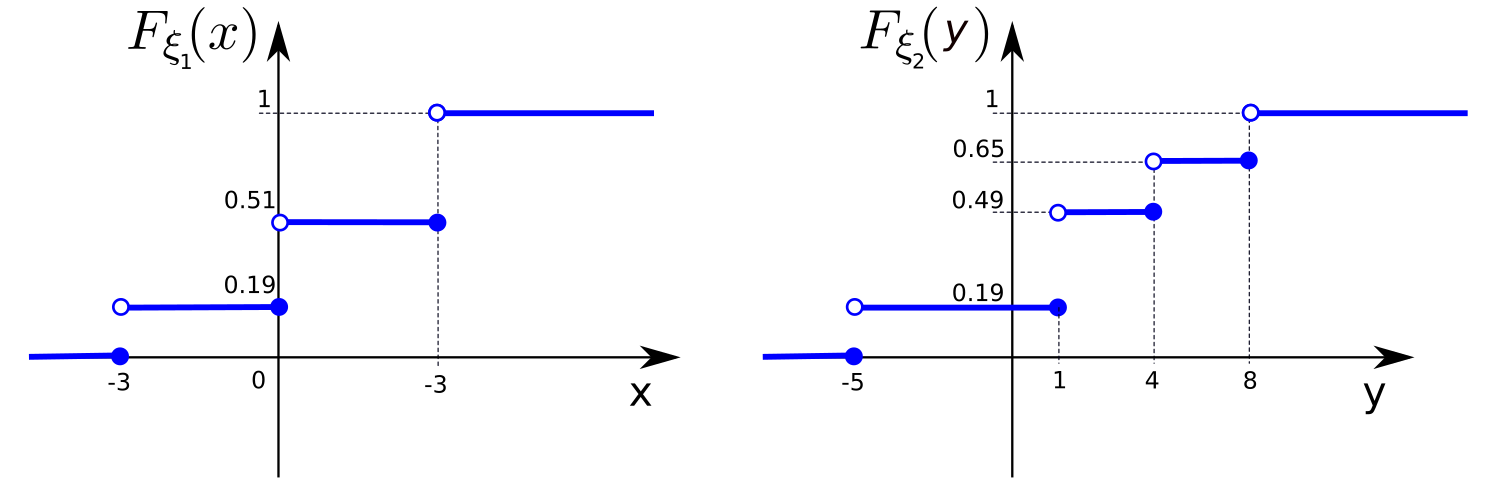
\includegraphics[scale=0.34]{assets/6.png} \end{center}

\def\Fx{F_{\overline{\xi}}}
\subsection{Сумісна функція розподілу випадкового вектора $\overline{\xi}$}

За означенням, $ F_{\overline{\xi}} (x,y) = \mathbb{P} \left\lbrace  \xi_1 < x, \xi_2 < y \right\rbrace$. Тоді $\Fx(x,y) = 0 $ якщо $\begin{gathered}
 x \leq x_1 \\
 y \leq y_1
\end{gathered}$.\\
Щоб полегшити знаходження $\Fx (x,y)$ намалюємо в декартовій
системі координат усі точки, що
відповідають значенню вектора $ \overline{\xi}$ та обчислимо значення
сумісної функції розподілу в кожній
області $D_{i,k}, i = \overline{1,3}, j = \overline{1,4}$.
\begin{center} 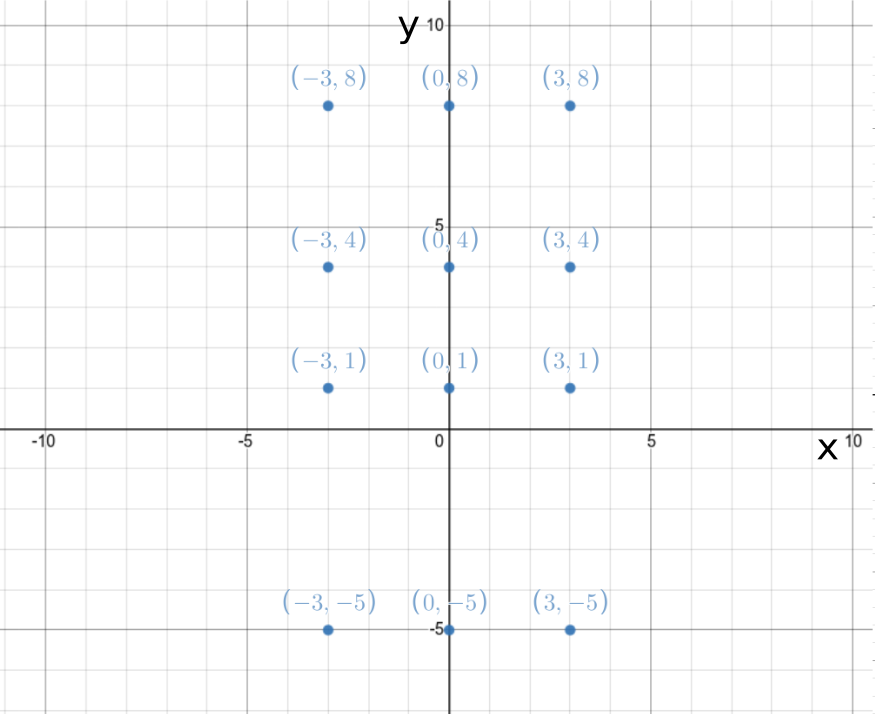
\includegraphics[scale=0.5]{assets/5.png} \end{center}
Використаємо формулу $ \Fx (x,y ) =  \sum\limits_{i: x_i < x}^{}{ \sum\limits_{j: y_j < y}^{}{ p_{ij}}}$.
$$
\begin{gathered}
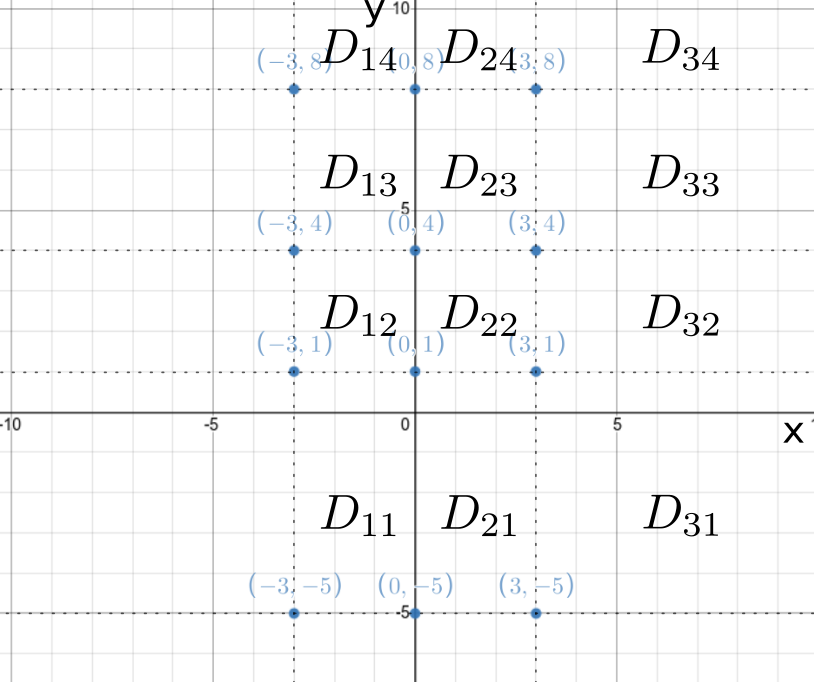
\includegraphics[scale=0.23]{assets/zonesD.png}
\end{gathered}\qquad
\begin{gathered}
 \text{Будемо почергово розглядати зони,}\\ \text{ як на малюнку зліва.}\\
 \\
 1. (x \leq -3) \lor (y\leq -5);\\
 \Fx (x,y) = 0
\end{gathered}
$$

$$ \begin{gathered}
2 .
D_{ 1 , 1 } =
\left\lbrace (x,y) \Bigg| \begin{gathered} -3  < x
\leq 0
\\ -5 < y
\leq 1
\end{gathered} \right\rbrace;\\
\Fx (x,y) =  \mathbb{P} \left\lbrace \xi_1 =-3, \xi_2 =-5\right\rbrace
= 0.06
\end{gathered}
\qquad
\begin{gathered}
 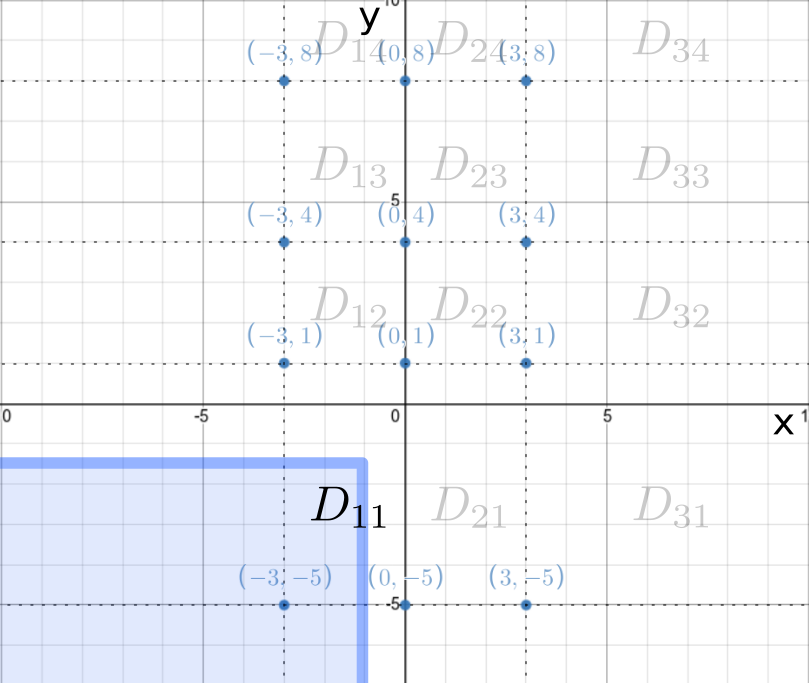
\includegraphics[scale=0.25]{assets/d11.png}
\end{gathered}
$$
$$ \begin{gathered}
3 .
D_{ 1 , 2 } =
\left\lbrace (x,y) \Bigg| \begin{gathered} -3  < x
\leq 0
\\ 1 < y
\leq 4
\end{gathered} \right\rbrace;\\
\Fx (x,y) =  \mathbb{P} \left\lbrace \xi_1 =-3, \xi_2 =-5\right\rbrace+\\+\mathbb{P} \left\lbrace \xi_1 =-3, \xi_2 =1\right\rbrace
= \\ =  0.06 + 0.04 = 0.1
\end{gathered}
\qquad\qquad
\begin{gathered}
 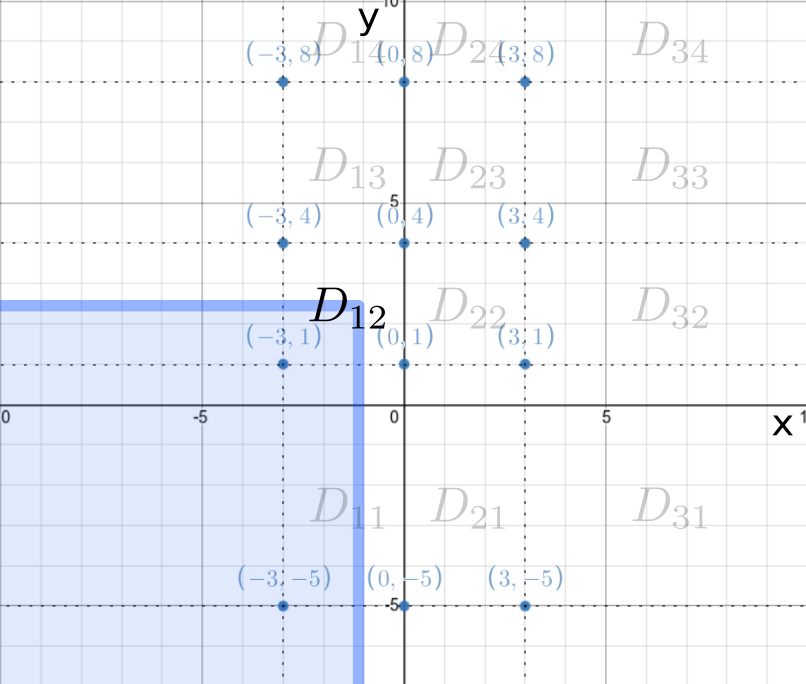
\includegraphics[scale=0.25]{assets/d12.png}
\end{gathered}
$$
$$ \begin{gathered}
4 .
D_{ 1 , 3 } =
\left\lbrace (x,y) \Bigg| \begin{gathered} -3  < x
\leq 0
\\ 4 < y
\leq 8
\end{gathered} \right\rbrace;\\
\Fx (x,y) =  \mathbb{P} \left\lbrace \xi_1 =-3, \xi_2 =-5\right\rbrace+\\+\mathbb{P} \left\lbrace \xi_1 =-3, \xi_2 =1\right\rbrace+\\+\mathbb{P} \left\lbrace \xi_1 =-3, \xi_2 =4\right\rbrace
= \\ =  0.06 + 0.04 + 0.06 = 0.16
\end{gathered}
\qquad\qquad
\begin{gathered}
 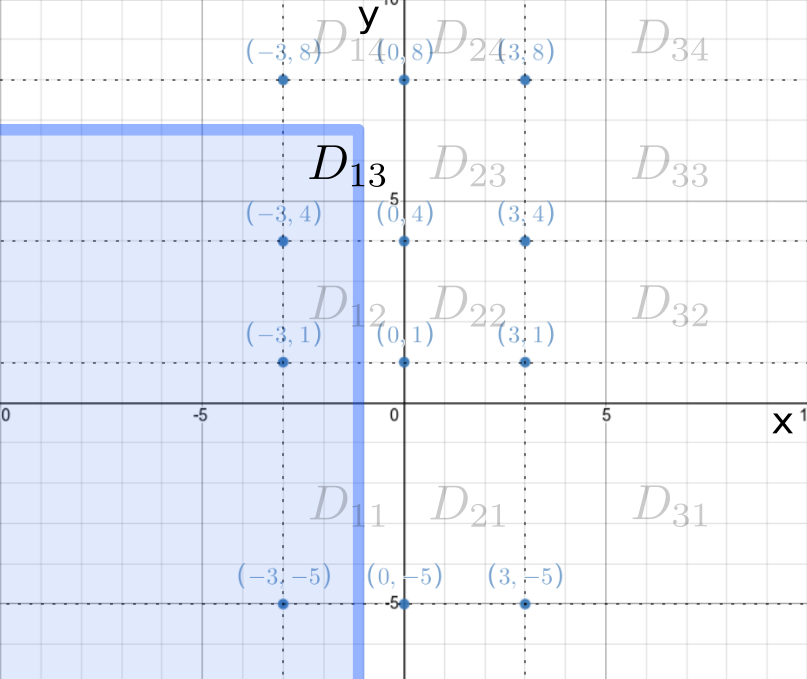
\includegraphics[scale=0.25]{assets/d13.png}
\end{gathered}
$$
$$ \begin{gathered}
5 .
D_{ 1 , 4 } =
\left\lbrace (x,y) \Bigg| \begin{gathered} -3  < x
\leq 0
\\ 8 < y
\end{gathered} \right\rbrace;\\
\Fx (x,y) =  \mathbb{P} \left\lbrace \xi_1 =-3, \xi_2 =-5\right\rbrace+\\+\mathbb{P} \left\lbrace \xi_1 =-3, \xi_2 =1\right\rbrace+\\+\mathbb{P} \left\lbrace \xi_1 =-3, \xi_2 =4\right\rbrace+\\+\mathbb{P} \left\lbrace \xi_1 =-3, \xi_2 =8\right\rbrace
= \\ =  0.06 + 0.04 +\\+ 0.06 + 0.03 = 0.19
\end{gathered}
\qquad\qquad
\begin{gathered}
 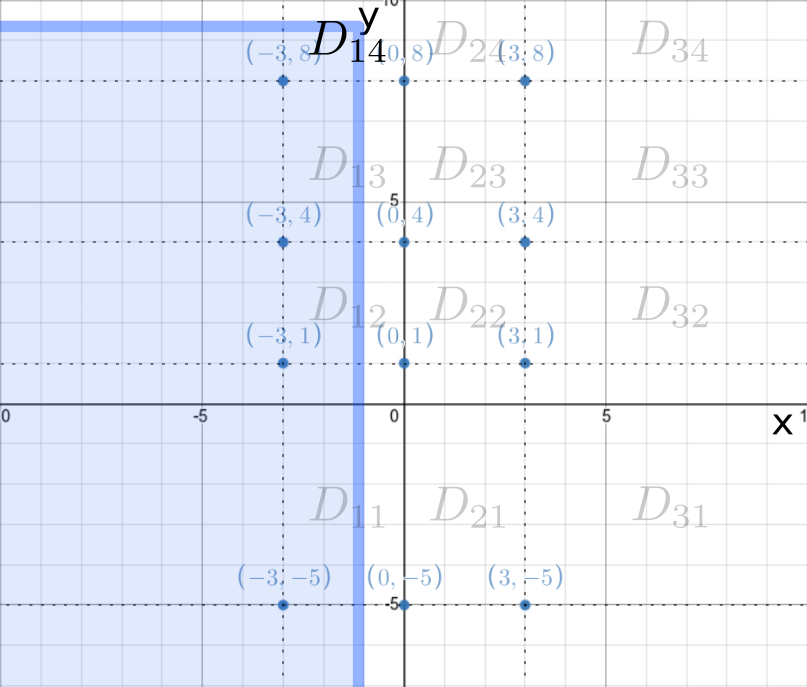
\includegraphics[scale=0.25]{assets/d14.png}
\end{gathered}
$$
$$ \begin{gathered}
6 .
D_{ 2 , 1 } =
\left\lbrace (x,y) \Bigg| \begin{gathered} 0  < x
\leq 3
\\ -5 < y
\leq 1
\end{gathered} \right\rbrace;\\
\Fx (x,y) =  \mathbb{P} \left\lbrace \xi_1 =-3, \xi_2 =-5\right\rbrace+\\+\mathbb{P} \left\lbrace \xi_1 =0, \xi_2 =-5\right\rbrace
= \\ =  0.06 + 0.01 = 0.07
\end{gathered}
\qquad\qquad
\begin{gathered}
 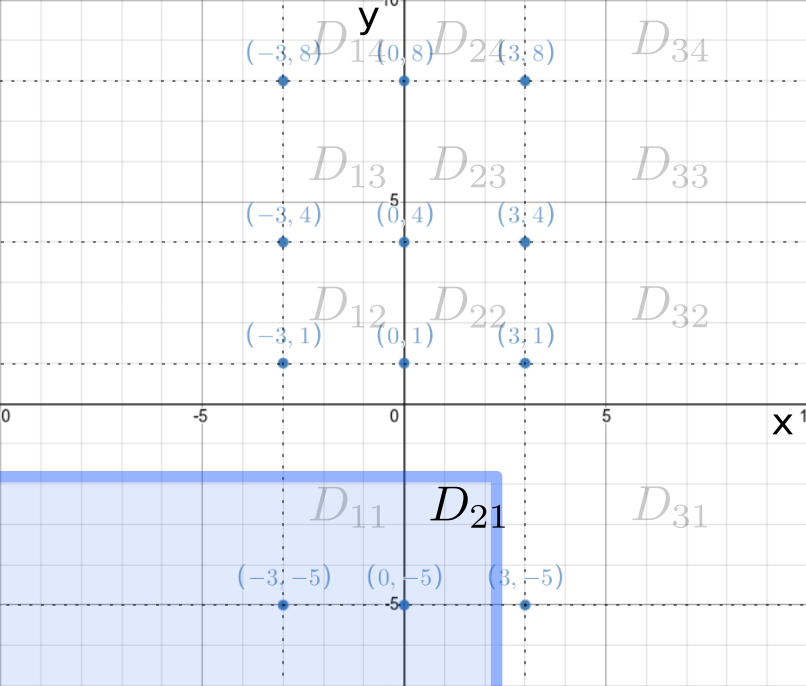
\includegraphics[scale=0.25]{assets/d21.png}
\end{gathered}
$$
$$ \begin{gathered}
7 .
D_{ 2 , 2 } =
\left\lbrace (x,y) \Bigg| \begin{gathered} 0  < x
\leq 3
\\ 1 < y
\leq 4
\end{gathered} \right\rbrace;\\
\Fx (x,y) =  \mathbb{P} \left\lbrace \xi_1 =-3, \xi_2 =-5\right\rbrace+\\+\mathbb{P} \left\lbrace \xi_1 =-3, \xi_2 =1\right\rbrace+\\+\mathbb{P} \left\lbrace \xi_1 =0, \xi_2 =-5\right\rbrace+\\+\mathbb{P} \left\lbrace \xi_1 =0, \xi_2 =1\right\rbrace
= \\ =  0.06 + 0.04 + 0.01 + 0.14 = 0.25
\end{gathered}
\qquad\qquad
\begin{gathered}
 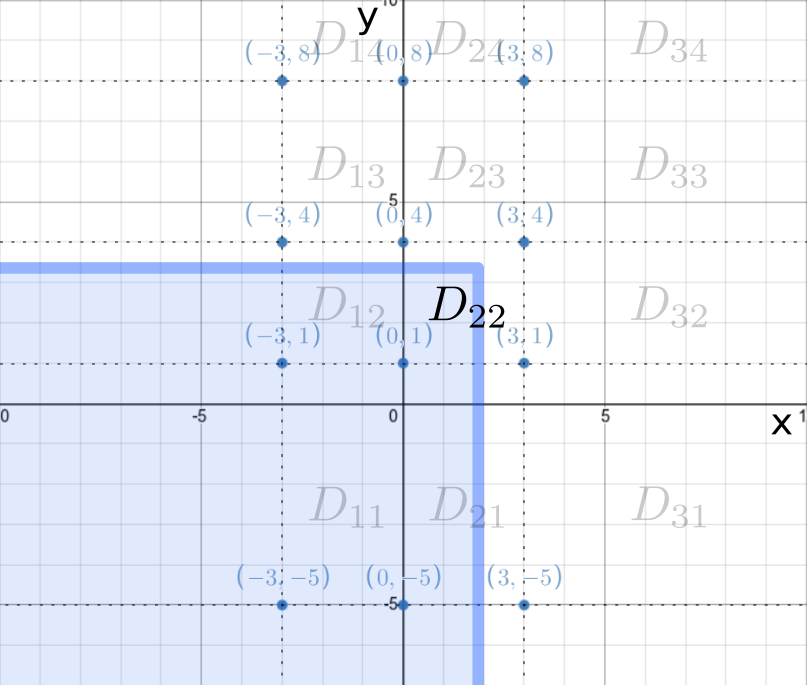
\includegraphics[scale=0.25]{assets/d22.png}
\end{gathered}
$$
$$ \begin{gathered}
8 .
D_{ 2 , 3 } =
\left\lbrace (x,y) \Bigg| \begin{gathered} 0  < x
\leq 3
\\ 4 < y
\leq 8
\end{gathered} \right\rbrace;\\
\Fx (x,y) =  \mathbb{P} \left\lbrace \xi_1 =-3, \xi_2 =-5\right\rbrace+\\+\mathbb{P} \left\lbrace \xi_1 =-3, \xi_2 =1\right\rbrace+\\+\mathbb{P} \left\lbrace \xi_1 =-3, \xi_2 =4\right\rbrace+\\+\mathbb{P} \left\lbrace \xi_1 =0, \xi_2 =-5\right\rbrace+\\+\mathbb{P} \left\lbrace \xi_1 =0, \xi_2 =1\right\rbrace+\\+\mathbb{P} \left\lbrace \xi_1 =0, \xi_2 =4\right\rbrace
= \\ =  0.06 + 0.04 + 0.06 +\\+ 0.01 + 0.14 + 0.04 = 0.35
\end{gathered}
\qquad\qquad
\begin{gathered}
 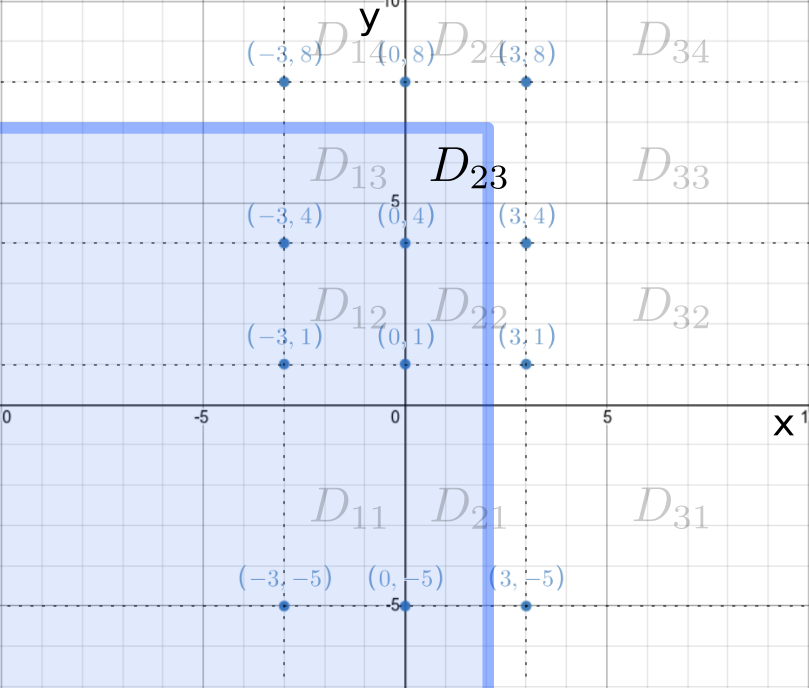
\includegraphics[scale=0.25]{assets/d23.png}
\end{gathered}
$$
$$ \begin{gathered}
9 .
D_{ 2 , 4 } =
\left\lbrace (x,y) \Bigg| \begin{gathered} 0  < x
\leq 3
\\ 8 < y
\end{gathered} \right\rbrace;\\
\Fx (x,y) =  \mathbb{P} \left\lbrace \xi_1 =-3, \xi_2 =-5\right\rbrace+\\+\mathbb{P} \left\lbrace \xi_1 =-3, \xi_2 =1\right\rbrace+\\+\mathbb{P} \left\lbrace \xi_1 =-3, \xi_2 =4\right\rbrace+\\+\mathbb{P} \left\lbrace \xi_1 =-3, \xi_2 =8\right\rbrace+\\+\mathbb{P} \left\lbrace \xi_1 =0, \xi_2 =-5\right\rbrace+\\+\mathbb{P} \left\lbrace \xi_1 =0, \xi_2 =1\right\rbrace+\\+\mathbb{P} \left\lbrace \xi_1 =0, \xi_2 =4\right\rbrace+\\+\mathbb{P} \left\lbrace \xi_1 =0, \xi_2 =8\right\rbrace
= \\ =  0.06 + 0.04 + 0.06 +\\+ 0.03 + 0.01 + 0.14 +\\+ 0.04 + 0.13 = 0.51
\end{gathered}
\qquad\qquad
\begin{gathered}
 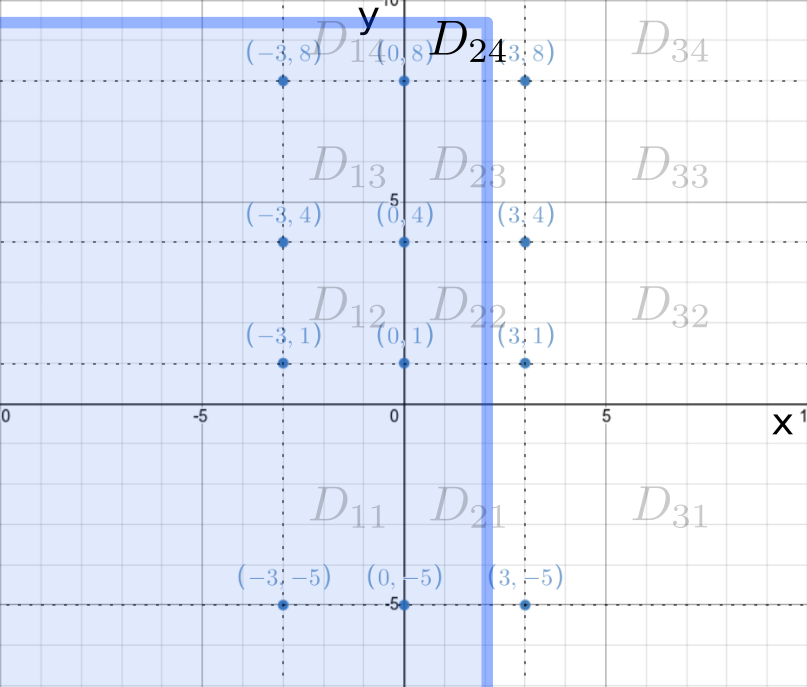
\includegraphics[scale=0.25]{assets/d24.png}
 \end{gathered}
$$
$$ \begin{gathered}
10 .
D_{ 3 , 1 } =
\left\lbrace (x,y) \Bigg| \begin{gathered} 3  < x
\\ -5 < y
\leq 1
\end{gathered} \right\rbrace;\\
\Fx (x,y) =  \mathbb{P} \left\lbrace \xi_1 =-3, \xi_2 =-5\right\rbrace+\\+\mathbb{P} \left\lbrace \xi_1 =0, \xi_2 =-5\right\rbrace+\\+\mathbb{P} \left\lbrace \xi_1 =3, \xi_2 =-5\right\rbrace
= \\ =  0.06 + 0.01 + 0.12 = 0.19
\end{gathered}
\qquad\qquad
\begin{gathered}
 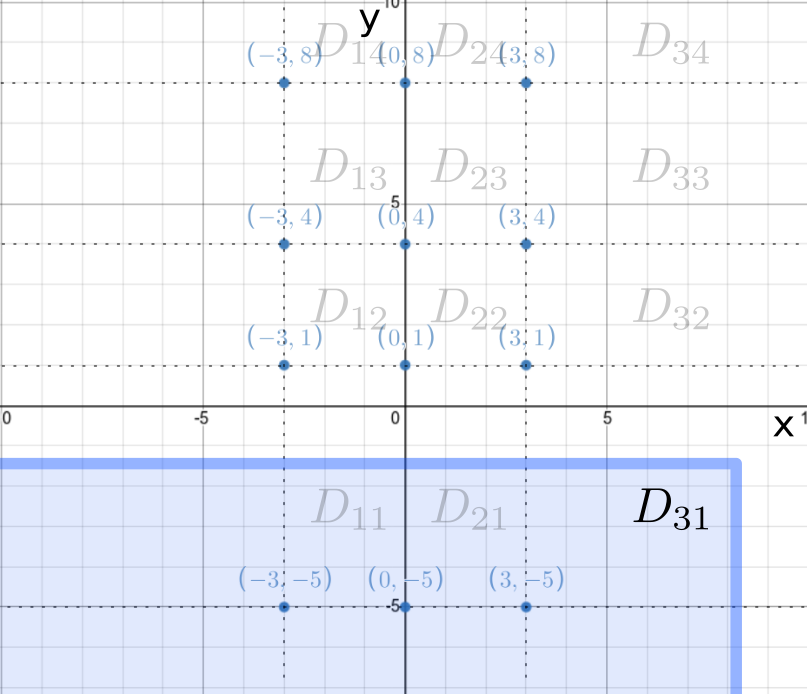
\includegraphics[scale=0.25]{assets/d31.png}
 \end{gathered}
$$
$$ \begin{gathered}
11 .
D_{ 3 , 2 } =
\left\lbrace (x,y) \Bigg| \begin{gathered} 3  < x
\\ 1 < y
\leq 4
\end{gathered} \right\rbrace;\\
\Fx (x,y) =  \mathbb{P} \left\lbrace \xi_1 =-3, \xi_2 =-5\right\rbrace+\\+\mathbb{P} \left\lbrace \xi_1 =-3, \xi_2 =1\right\rbrace+\\+\mathbb{P} \left\lbrace \xi_1 =0, \xi_2 =-5\right\rbrace+\\+\mathbb{P} \left\lbrace \xi_1 =0, \xi_2 =1\right\rbrace+\\+\mathbb{P} \left\lbrace \xi_1 =3, \xi_2 =-5\right\rbrace+\\+\mathbb{P} \left\lbrace \xi_1 =3, \xi_2 =1\right\rbrace
= \\ =  0.06 + 0.04 + 0.01 + 0.14 +\\+ 0.12 + 0.12 = 0.49
\end{gathered}
\qquad\qquad
\begin{gathered}
 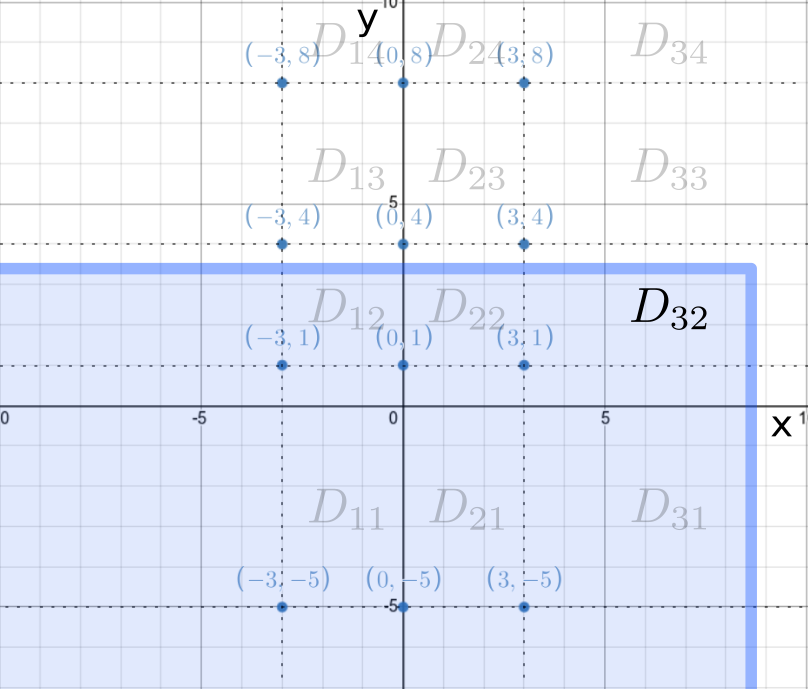
\includegraphics[scale=0.25]{assets/d32.png}
 \end{gathered}
$$
$$ \begin{gathered}
12 .
D_{ 3 , 3 } =
\left\lbrace (x,y) \Bigg| \begin{gathered} 3  < x
\\ 4 < y
\leq 8
\end{gathered} \right\rbrace;\\
\Fx (x,y) =  \mathbb{P} \left\lbrace \xi_1 =-3, \xi_2 =-5\right\rbrace+\\+\mathbb{P} \left\lbrace \xi_1 =-3, \xi_2 =1\right\rbrace+\\+\mathbb{P} \left\lbrace \xi_1 =-3, \xi_2 =4\right\rbrace+\\+\mathbb{P} \left\lbrace \xi_1 =0, \xi_2 =-5\right\rbrace+\\+\mathbb{P} \left\lbrace \xi_1 =0, \xi_2 =1\right\rbrace+\\+\mathbb{P} \left\lbrace \xi_1 =0, \xi_2 =4\right\rbrace+\\+\mathbb{P} \left\lbrace \xi_1 =3, \xi_2 =-5\right\rbrace+\\+\mathbb{P} \left\lbrace \xi_1 =3, \xi_2 =1\right\rbrace+\\+\mathbb{P} \left\lbrace \xi_1 =3, \xi_2 =4\right\rbrace
= \\ =  0.06 + 0.04 + 0.06 + 0.01 +\\+ 0.14 + 0.04 + 0.12 +\\+ 0.12 + 0.06 = 0.65
\end{gathered}
\qquad\qquad
\begin{gathered}
 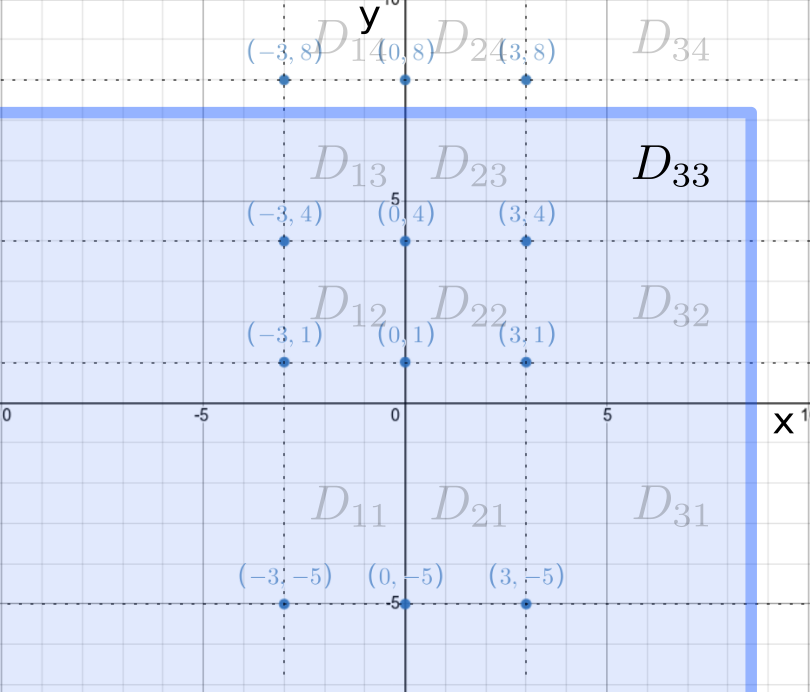
\includegraphics[scale=0.25]{assets/d33.png}
 \end{gathered}
$$
$$ \begin{gathered}
13 .
D_{ 3 , 4 } =
\left\lbrace (x,y) \Bigg| \begin{gathered} 3  < x
\\ 8 < y
\end{gathered} \right\rbrace;\\
\Fx (x,y) =  \mathbb{P} \left\lbrace \xi_1 =-3, \xi_2 =-5\right\rbrace+\\+\mathbb{P} \left\lbrace \xi_1 =-3, \xi_2 =1\right\rbrace+\\+\mathbb{P} \left\lbrace \xi_1 =-3, \xi_2 =4\right\rbrace+\\+\mathbb{P} \left\lbrace \xi_1 =-3, \xi_2 =8\right\rbrace+\\+\mathbb{P} \left\lbrace \xi_1 =0, \xi_2 =-5\right\rbrace+\\+\mathbb{P} \left\lbrace \xi_1 =0, \xi_2 =1\right\rbrace+\\+\mathbb{P} \left\lbrace \xi_1 =0, \xi_2 =4\right\rbrace+\\+\mathbb{P} \left\lbrace \xi_1 =0, \xi_2 =8\right\rbrace+\\+\mathbb{P} \left\lbrace \xi_1 =3, \xi_2 =-5\right\rbrace+\\+\mathbb{P} \left\lbrace \xi_1 =3, \xi_2 =1\right\rbrace+\\+\mathbb{P} \left\lbrace \xi_1 =3, \xi_2 =4\right\rbrace+\\+\mathbb{P} \left\lbrace \xi_1 =3, \xi_2 =8\right\rbrace
= \\ =  0.06 + 0.04 + 0.06 + 0.03 +\\+ 0.01 + 0.14 + 0.04 + 0.13 +\\+ 0.12 + 0.12 + 0.06 + 0.19 = 1
\end{gathered}
\qquad\qquad
\begin{gathered}
 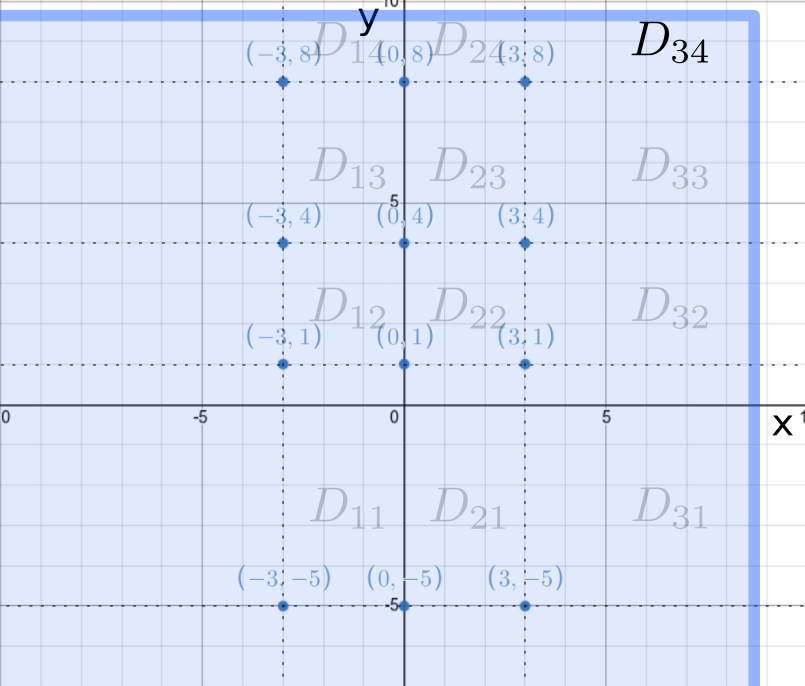
\includegraphics[scale=0.25]{assets/d34.png}
 \end{gathered}
$$
\vfill
Отримали сумісну функцію розподілу, яку можна записати у вигляді
таблиці.
$$
\begin{tabular}{|c|c|c|c|c|}
\hline
$y \setminus x$ & $x \leq -3$ & $-3 < x \leq 0$ & $0 < x \leq 3$ & $3 < x$ \\ \hline
$y\leq -5$      & 0           & 0               & 0              & 0       \\ \hline
$-5< y\leq1$    & 0           & 0.06            & 0.07           & 0.19    \\ \hline
$1< y\leq4$     & 0           & 0.10            & 0.25           & 0.49    \\ \hline
$4< y\leq8$     & 0           & 0.16            & 0.35           & 0.65    \\ \hline
$8< y$          & 0           & 0.19            & 0.51           & 1.00    \\ \hline
\end{tabular}
$$
Перевірка: (властивість узгодження)\\
$
 \lim\limits_{x\to  +\infty}{ \Fx (x,y) = F_{\xi_2} (y)}
$ - виконується, адже в останньому стовпчику $F_{\xi_2} (y)$.\\
$ \lim\limits_{y\to  +\infty}{\Fx (x,y)} = F_{\xi_1}(x) $ -
 иконується, адже в останній стрічці $F_{\xi_1} (x)$.\\
 $\lim\limits_{\substack{%
     a \to -\infty\\
     b \to \infty}}{ \Fx (x,y)} = 1 $ \quad $\Fx (x,y) = 1 \quad \forall (x,y) \in D_{3,4}$
 \vfill

\newpage
Або у вигляді сукупності:
$$
\Fx(x,y) = \begin{cases}
0,\quad& (x \leq -3) \lor (y\leq -5);\\
0.06, \quad&(-3 < x \leq 0)\land (-5< y\leq1);\\
0.1, \quad&(-3 < x \leq 0)\land (1< y\leq4);\\
0.16, \quad&(-3 < x \leq 0)\land (4< y\leq8);\\
0.19, \quad&(-3 < x \leq 0)\land (8< y);\\
0.07, \quad&(0 < x \leq 3)\land (-5< y\leq1);\\
0.25, \quad&(0 < x \leq 3)\land (1< y\leq4);\\
0.35, \quad&(0 < x \leq 3)\land (4< y\leq8);\\
0.51, \quad&(0 < x \leq 3)\land (8< y);\\
0.19, \quad&(3 < x )\land (-5< y\leq1);\\
0.49, \quad&(3 < x )\land (1< y\leq4);\\
0.65, \quad&(3 < x )\land (4< y\leq8);\\
1, \quad&(3 < x )\land (8< y);
\end{cases}
$$

\subsection{Математичні
сподівання
координат.
Кореляційна
та
нормована кореляційна матриця.}

а) За рядом розподілу величини $\xi_1$ знайдемо математичне сподівання:

$$
\mathbb{E}\xi_1 =  \sum\limits_{i = 1}^{ 3}{ x_i p_{i}} = -3 * 0.19 + 0*0.32 + 3*0.49 =0.9
$$
Аналогічно для $\xi_2$:
$$
\mathbb{E}\xi_2 =  \sum\limits_{j = 1}^{ 4}{ y_j p_{j}} = -5*0.19 + 1*0.3 + 4 * 0.16 + 8*0.35 = 2.79
$$
Центр розсіювання вектора $\overline{\xi} - (0.9, 2.79)$\\
б) Побудуємо кореляційну та нормовану кореляційну матриці.\\
Для дискретного вектора:
$$
cov( \xi_1, \xi_2) = \sum\limits_{i = 1}^{ m}{
 \sum\limits_{j = 1}^{ n}{ x_i \cdot y_j \cdot p_{ij}}
} - \left\lbrace  \sum\limits_{i = 1}^{ m}{
 \sum\limits_{j = 1}^{ n}{ x_i p_{ij}}
} \right\rbrace
\cdot
\left\lbrace \sum\limits_{i = 1}^{ m}{
 \sum\limits_{j = 1}^{ n}{ y_j p_{ij}}
} \right\rbrace
$$
$$
C_{ \overline{\xi}} = \begin{bmatrix}
 \mathbb{D}\xi_1 & cov(\xi_1, \xi_2) \\
 cov(\xi_1, \xi_2) & \mathbb{D} \xi_2
\end{bmatrix}
$$

Розрахуємо та внесемо до матриці всі необхідні величини:
$$
\begin{gathered}
cov(\xi_1, \xi_2)= ( (-3) \cdot (-5) \cdot 0.06 )
+( (-3) \cdot 1 \cdot 0.04 )
+( (-3) \cdot 4 \cdot 0.06 )
+\\+( (-3) \cdot 8 \cdot 0.03 )
+( 0 \cdot (-5) \cdot 0.01 )
+( 0 \cdot 1 \cdot 0.14 )
+\\+( 0 \cdot 4 \cdot 0.04 )
+( 0 \cdot 8 \cdot 0.13 )
+( 3 \cdot (-5) \cdot 0.12 )
+\\+( 3 \cdot 1 \cdot 0.12 )
+( 3 \cdot 4 \cdot 0.06 )
+( 3 \cdot 8 \cdot 0.19 ) - \mathbb{E}\xi_1 \cdot\mathbb{E}\xi_2=\\
= 0.9 -0.12 -0.72 -0.72 -1.8+ 0.36+ 0.72+ 4.56 - 2.511=  0.669
\end{gathered}
$$
Знайдемо дисперсію компонент $\xi_1$ та $\xi_2$:
$$
\mathbb{D}\xi_1 = \mathbb{E}\xi_1^2 - (\mathbb{E}\xi_1)^2 =  \sum\limits_{i = 1}^{ 3}{x_i^2 \cdot p_i} - 0.9^2 =  6.12 - 0.81 = 5.31
$$
$$
\mathbb{D}\xi_2 = \mathbb{E}\xi_2^2 - (\mathbb{E}\xi_2)^2 =  \sum\limits_{j = 1}^{ 4}{y_j^2 \cdot p_j} - 2.79^2 =  30.01 - 7.7841 = 22.2259
$$
Отримали кореляційну матрицю:
$$
C_{\overline{\xi}} = \begin{bmatrix}
 5.31 & 0.669\\
 0.669 & 22.2259
\end{bmatrix}
$$
Оскільки $cov(\xi_1, \xi_2)> 0$ випадкові величини $\xi_1,  \xi_2$ є корельованими та залежними.
Перевіримо додатну визначеність $C_{\overline{\xi}}$:
$$\det C_{\overline{\xi}} =5.31 \cdot 22.2259 - 0.669^2 = 117.571968 >0$$
Знайдемо коефіцієнт кореляції: $r_{\overline{\xi}} = \dfrac{cov(\xi_1, \xi_2)}{\sqrt{\mathbb{D}\xi_1\cdot \mathbb{D}\xi_2}} \approx \dfrac{0.669 }{ \sqrt{118.02}} \approx 0.0616 $

\subsection{Умовні ряди розподілу для кожної координати.}
Обчислимо умовні ймовірності:
$$
\mathbb{P} \left\lbrace \xi_1 = x_i | \xi_2 = y_j \right\rbrace = \frac{\mathbb{P} \left\lbrace \xi_1 = x_i , \xi_2 = y_j \right\rbrace}{\mathbb{P} \left\lbrace \xi_2 = y_j \right\rbrace} = \frac{p_{ij}}{p_j}
$$
$$
\mathbb{P} \left\lbrace \xi_2 = y_j | \xi_1  = x_i \right\rbrace = \frac{\mathbb{P} \left\lbrace \xi_1 = x_i, \xi_2 = y_j \right\rbrace}{\mathbb{P} \left\lbrace \xi_1 = x_i \right\rbrace}= \frac{p_{ij}}{p_i}
$$
Обчислюємо умовні ряди розподілу для
$\xi_1$ та
$\xi_2$
та результати
заносимо у таблиці. Отримані дроби скорочуємо, але для
зручності у кожному рядку залишаємо однаковий знаменник.\\
Умовні ряди розподілу $\xi_1$:
$$
\begin{tabular}{|c|c|c|c|}
\hline
$\xi_1$ & -3 & 0 & 3 \\ \hline
$\mathbb{P} \left\lbrace \xi_1 = x_i | \xi_2 = -5  \right\rbrace$ & $6/19$ & $1/19$ & $12/19$ \\ \hline
$\mathbb{P} \left\lbrace \xi_1 = x_i | \xi_2 = 1  \right\rbrace$ & $4/30$ & $14/30$ & $12/30$ \\ \hline
$\mathbb{P} \left\lbrace \xi_1 = x_i | \xi_2 = 4  \right\rbrace$ & $6/16$ & $4/16$ & $6/16$ \\ \hline
$\mathbb{P} \left\lbrace \xi_1 = x_i | \xi_2 = 8  \right\rbrace$ & $3/35$ & $13/35$ & $19/35$ \\ \hline
\end{tabular} \qquad \qquad
\begin{gathered}
\text{Перевірка:}\\ \frac{6}{19}+\frac{1}{19}+ \frac{12}{19}= 1\\
\frac{4}{30}+\frac{14}{30}+\frac{12}{30} = 1\\
\frac{6}{16}+\frac{4}{16}+\frac{6}{16} = 1\\
\frac{3}{35}+\frac{13}{35}+\frac{19}{35} = 1
\end{gathered}
$$


Умовні ряди розподілу $\xi_2$:
$$
\begin{tabular}{|c|c|c|c|c|}
\hline
$\xi_2$ & -5 & 1 & 4 & 8 \\ \hline
$\mathbb{P} \left\lbrace \xi_2 = y_j | \xi_1 = -3  \right\rbrace$ & 6/19 & 4/19 & 6/19 & 3/19 \\ \hline
$\mathbb{P} \left\lbrace \xi_2 =y_j | \xi_1 = 0  \right\rbrace$ & 1/32 & 14/32 & 4/32 & 13/32 \\ \hline
$\mathbb{P} \left\lbrace \xi_2 = y_j | \xi_1 = 3  \right\rbrace$ & 12/49 & 12/49 & 6/49 & 19/49 \\ \hline
\end{tabular} \qquad
\begin{gathered}
\text{Перевірка:}\\ \frac{6}{19}+\frac{4}{19}+ \frac{6}{19} + \frac{3}{19}  = 1\\
\frac{1}{32} + \frac{14}{32} + \frac{4}{32} + \frac{13}{32}  = 1\\
\frac{12}{49} + \frac{12}{49} + \frac{6}{49} + \frac{19}{49}     = 1
\end{gathered}
$$
\subsection{Умовні математичні сподівання для кожної координати з
перевіркою.}
Скористаємося формулами:
$$
\mathbb{E}(\xi_1 | \xi_2 =  y_j) =  \sum\limits_{i = 1}^{ 3}{ x_i \cdot \mathbb{P} \left\lbrace \xi_1 = x_i | \xi_2 = y_j \right\rbrace}
$$
$$
\mathbb{E}(\xi_2 | \xi_1 = x_i) =  \sum\limits_{j = 1}^{ 4}{ y_j  \cdot\mathbb{P} \left\lbrace \xi_2 = y_j | \xi_1 = x_i \right\rbrace}
$$
Обчислимо ряд розподілу $\mathbb{E}(\xi_1| \xi_2)$:
$$
\mathbb{E}(\xi_1| \xi_2 = -5) = (-3)\cdot\frac{6}{19}+0\cdot\frac{1}{19}+ 3\cdot\frac{12}{19} = \frac{18}{19}
$$
$$
\mathbb{E}(\xi_1| \xi_2 = 1) = (-3)\cdot\frac{4}{30}+0\cdot\frac{14}{30}+3\cdot\frac{12}{30} = \frac{24}{30} = \frac{12}{15}
$$
$$
\mathbb{E}(\xi_1| \xi_2 = 4) = (-3)\cdot\frac{6}{16}+0\cdot\frac{4}{16}+3\cdot\frac{6}{16} = 0
$$
$$
\mathbb{E}(\xi_1| \xi_2 = 8) = (-3)\cdot\frac{3}{35}+0\cdot\frac{13}{35}+3\cdot\frac{19}{35} = \frac{48}{35}
$$
Перевіримо за формулою повного математичного сподівання:
$$\begin{gathered}
 \mathbb{E}(\mathbb{E}(\xi_1 | \xi_2)) = 0.19\cdot\frac{18}{19} + 0.3 \cdot \frac{12}{15}  + 0.16\cdot 0 + 0.35 \cdot \frac{48}{35}  =\\ = 0.18 +  0.24 +0+ 0.48 = 0.9 = \mathbb{E} \xi_1
\end{gathered}$$
Обчислимо ряд розподілу $\mathbb{E}(\xi_2 | \xi_1)$:
$$
\begin{gathered}
\mathbb{E}(\xi_2| \xi_1 = -3) = (-5)\cdot\frac{6}{19}+ 1\cdot\frac{4}{19}+ 4\cdot\frac{6}{19} + 8\cdot\frac{3}{19}  = \frac{22}{19} \\
\mathbb{E}(\xi_2| \xi_1 = 0) =(-5)\cdot\frac{1}{32} + 1\cdot\frac{14}{32} + 4\cdot\frac{4}{32} + 8\cdot\frac{13}{32}  = \frac{129}{32} \\
\mathbb{E}(\xi_2| \xi_1 = 3) =(-5)\cdot\frac{12}{49} + 1\cdot\frac{12}{49} + 4\cdot\frac{6}{49} + 8\cdot\frac{19}{49} = \frac{128}{49}
\end{gathered}
$$
Перевіримо за формулою повного математичного сподівання:
$$
\mathbb{E}(\mathbb{E}(\xi_2 | \xi_1)) = 0.19 \cdot \frac{22}{19} + 0.32 \cdot \frac{129}{32} + 0.49 \cdot \frac{128}{49} = \\ = 0.22 + 1.29 + 1.28 = 2.79 = \mathbb{E}\xi_2
$$
Отримали такі умовні ряди розподілу для $\mathbb{E}(\xi_2 | \xi_1)$ , $\mathbb{E}(\xi_2 | \xi_1)$:
\begin{center}
\begin{tabular}{|c|c|c|c|}
\hline
$\mathbb{E}(\xi_2| \xi_1)$ & 22/19 & 129/32 & 128/49 \\ \hline
P & 0.19 & 0.32 & 0.49 \\ \hline
\end{tabular} \qquad
\begin{tabular}{|c|c|c|c|c|}
\hline
$\mathbb{E}(\xi_1| \xi_2)$ & 18/19 & 12/15 & 0 & 48/35 \\ \hline
P       & 0.19  & 0.3 & 0.16 & 0.35 \\ \hline
\end{tabular}
\end{center}

\newpage

\section{Завдання 2}
\vfill

Нехай неперервний
випадковий вектор $\overline{\xi} = \begin{bmatrix}
 \xi_1, \xi_2
\end{bmatrix}$ рівномірно розподілений в області $G$.
\begin{center} 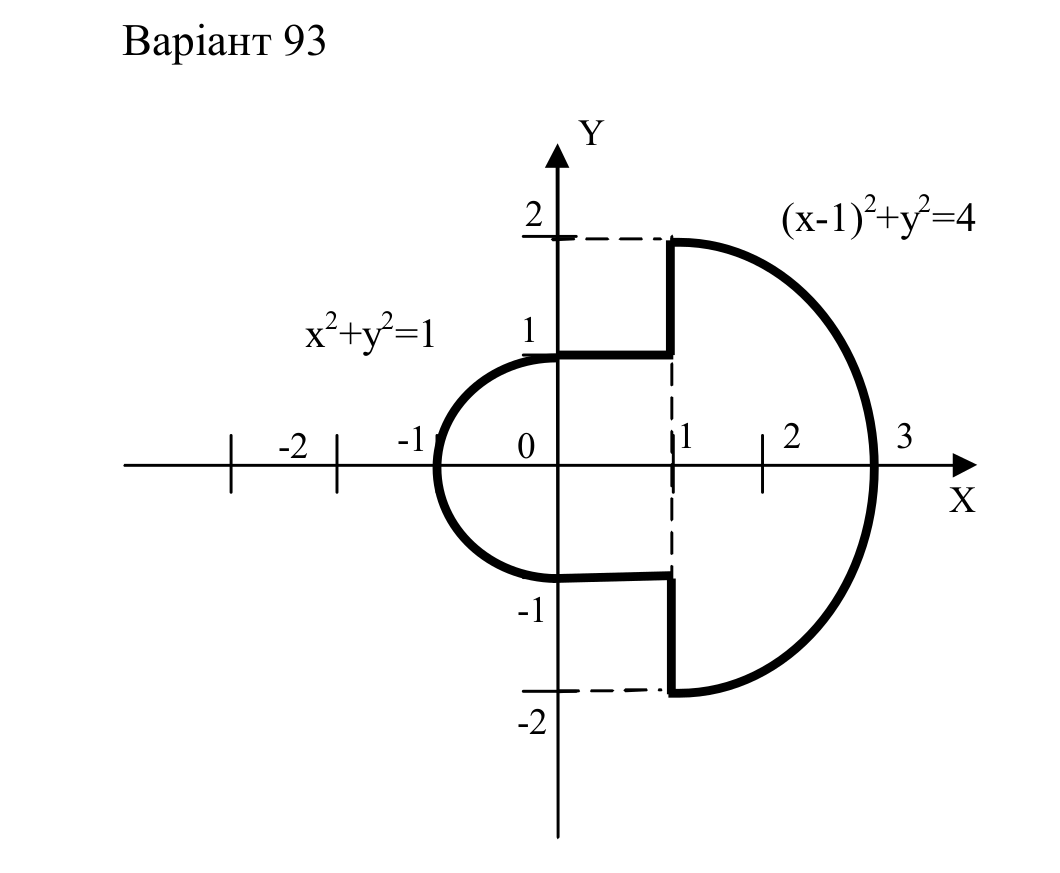
\includegraphics[scale=0.44]{assets/graph2.png} \end{center}
\vfill

Центр півкола $x^2 + y^2 = 1$ - (0,0). Центр півкола $(x-1)^2 + y^2 = 4$ - (1, 0). Усі рівняння кривих вказано на рисунку.\\
\vfill
Задану область можна розбити наступним чином:
$$G = \left\lbrace (x,y) \quad \Bigg| \quad
\begin{gathered}
  \left(
(-1 \leq x < 0) \land ( -\sqrt{1 -x^2} \leq y \leq  \sqrt{1-x^2})
\right)  \lor \\ \lor \left(
(0 \leq  x \leq 1) \land (-1 \leq y \leq 1)
	 \right)\lor \\ \lor \left(
(1 \leq  x\leq  3) \land (-\sqrt{4 -(x-1)^2}\leq  y \leq\sqrt{4 - (x-1)^2})
\right)
\end{gathered}    \right\rbrace  $$
\vfill

\newpage
\subsection{Щільності розподілу координат $\xi_1$ та  $\xi_2$}
Спочатку, знайдемо в загальному вигляді інтеграл:
$$
 \int\limits_{}^{}{\sqrt{a^2 - t^2}dt} = \left| \begin{gathered}
  \text{Заміна:}\\
	t = a\sin{(s)}\\
	dt = a \cos{(s)} ds
 \end{gathered} \right| =  a^2 \cdot \int\limits_{}^{}{\cos^2{(s)}ds } = a^2 \cdot \int{ \frac{\cos{(2s)}+1}{2} ds } =
$$
$$
= a^2 \cdot \frac{ \frac{\sin{(2s)} }{2} +s}{2} +C =   \frac{ t\sqrt{a^2 - t^2} +a^2\arcsin{\left( \frac{t}{a}  \right) }}{2} +C
$$
$$S_{G} =   \iint\limits_{G}{dxdy} =  \int\limits_{-1}^{ 0}{dx  \int\limits_{-\sqrt{1 -x^2}}^{ \sqrt{1 -x^2}}{dy}} +
 \int\limits_{0}^{1}{dx  \int\limits_{-1}^{ 1}{dy}} +  \int\limits_{1}^{3}{dx  \int\limits_{-\sqrt{4 -(x-1)^2}}^{ \sqrt{4 -(x-1)^2}}{dy}} = $$
 $$
 = 2  \int\limits_{-1}^{0}{ \sqrt{1 - x^2}dx} + 2 +  2\int\limits_{1}^{3}{\sqrt{4 -(x-1)^2}dx } = $$
 $$ =\left| \begin{gathered}
\text{У I інтегралі:} \\
 x = \sin{(t)} \Rightarrow dx = \cos{(t)}dt\\
t_2(0) = 0 \quad t_1 = -\frac{\pi}{2}
 \end{gathered} \qquad \quad \begin{gathered}\text{У II інтегралі:} \\
  x-1 = 2\sin{(t)} \Rightarrow dx = 2\cos{(t)}dt\\
  t_2 = \frac{\pi}{2}\quad  t_1(0) = 0
  \end{gathered}\right| =
 $$
$$
=  2\int\limits_{- \frac{\pi}{2} }^{0}{\cos^2{(t)}dt } + 8  \int\limits_{0}^{ \frac{\pi}{2} 	}{ \cos^2{(t)}dt } =
\left( \frac{\sin{(2t)}}{2}   + t  \right)  \Bigg|_{ -\frac{\pi}{2} }^0 + 2 + 4\cdot \left(  \frac{\sin{(2t)}}{2}   + t  \right) \Bigg|^{ \frac{\pi}{2} }_0 =
$$
$$
= 2\pi + \frac{\pi}{2} + 2 = 2.5 \pi + 2
$$
Тоді
щільність
вектора
рівномірно
розподіленого в області $G$:
\def\fx{f_{\overline{\xi}}}
$$
\fx  (x,y ) = \begin{cases}
	\dfrac{1}{ 2.5\pi + 2}, \quad&(x,y) \in G; \\
	0, \quad& (x,y) \notin G
\end{cases}
$$
Із визначення рівномірного розподілу випливає, що умова нормування для $\fx (x,y)$ виконана $ \left( \frac{1}{S_G}  * \iint\limits_{G}{dxdy} = (2.5\pi +2 )\cdot \dfrac{1}{2.5\pi + 2} =1 \right)$.\\
Обчислимо щільності координат вектора $\overline{\xi}$:
$$
f_{\xi_1} (x) =  \int\limits_{-\i}^{ +\infty}{ \fx (x,y) dy} \qquad f_{\xi_2}(y) =  \int\limits_{-\i}^{ +\infty}{ \fx (x,y) dx}
$$
$$
f_{\xi_1}(x) = \begin{cases}
0, \quad x \leq -1 ;\\
	\dfrac{1}{2.5\pi + 2}  \int\limits_{-\sqrt{(1-x^2)}}^{ \sqrt{(1-x^2)}}{dy} = \dfrac{2}{2.5\pi + 2} \sqrt{(1-x^2)}, \quad -1 < x \leq 0; \\
	\dfrac{1}{2.5\pi + 2}  \int\limits_{-1}^{ 1}{dy} = \dfrac{2}{2.5\pi + 2}, \quad 0 < x \leq 1; \\
	\dfrac{1}{2.5\pi + 2} \int\limits_{ -\sqrt{4 - (x-1)^2}}^{ \sqrt{4 - (x-1)^2}}{ dy} = \dfrac{2}{2.5\pi + 2} \sqrt{4 - (x-1)^2}, \quad 1 < x \leq 3; \\
	0, \quad x > 3 ;\\
\end{cases}
$$
Графік отриманої функції щільності:
\begin{center} 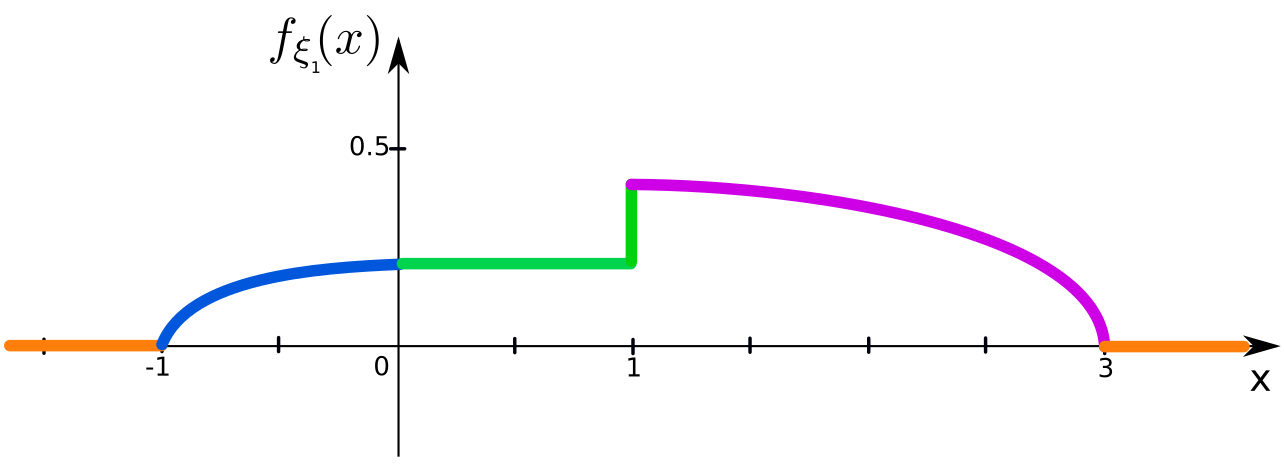
\includegraphics[scale=0.37]{assets/fxi11.png} \end{center}
Перевірка умови нормування:
$$
 \int\limits_{-\i}^{ +\infty}{ f_{\xi_1} (x) dx} = 0 + \frac{2}{2.5\pi + 2}  \cdot \left(
\int\limits_{-1}^{ 0}{ \sqrt{1-x^2}dx} +  \int\limits_{0}^{ 1}{dx} +  \int\limits_{1}^{ 3}{\sqrt{4 - (x-1)^2}dx}
  \right) =
$$
$$
=  \dfrac{2}{2.5\pi + 2} \cdot \frac{(2.5\pi +2 )}{2}  =1
$$
Зауваження. Вже знаходили ці інтеграли під час пошуку площі фігури.
$$
f_{\xi_2} (y) = \begin{cases}
	0, \quad y \leq  -2;\\
	\dfrac{1}{2.5\pi + 2}  \int\limits_{1}^{ 1+ \sqrt{4 - y^2}}{dx} = \dfrac{1}{2.5\pi + 2} \cdot \sqrt{4 - y^2}, \quad -2 < y \leq -1;\\
	\dfrac{1}{2.5\pi + 2}   \int\limits_{- \sqrt{1-y^2}}^{1+ \sqrt{4 - y^2}}{dx}
	=  \dfrac{1}{2.5\pi + 2} \cdot \left( \sqrt{4 - y^2} + \sqrt{1-y^2}+ 1  \right),  -1 < y \leq 1; \\
		\dfrac{1}{2.5\pi + 2}  \int\limits_{1}^{ 1+ \sqrt{4 - y^2}}{dx} = \dfrac{1}{2.5\pi + 2} \cdot \sqrt{4 - y^2}, \quad 1 < y \leq 2;\\
			0, \quad y >  2;\\
\end{cases}
$$
Графік отриманої функції щільності:
\begin{center} 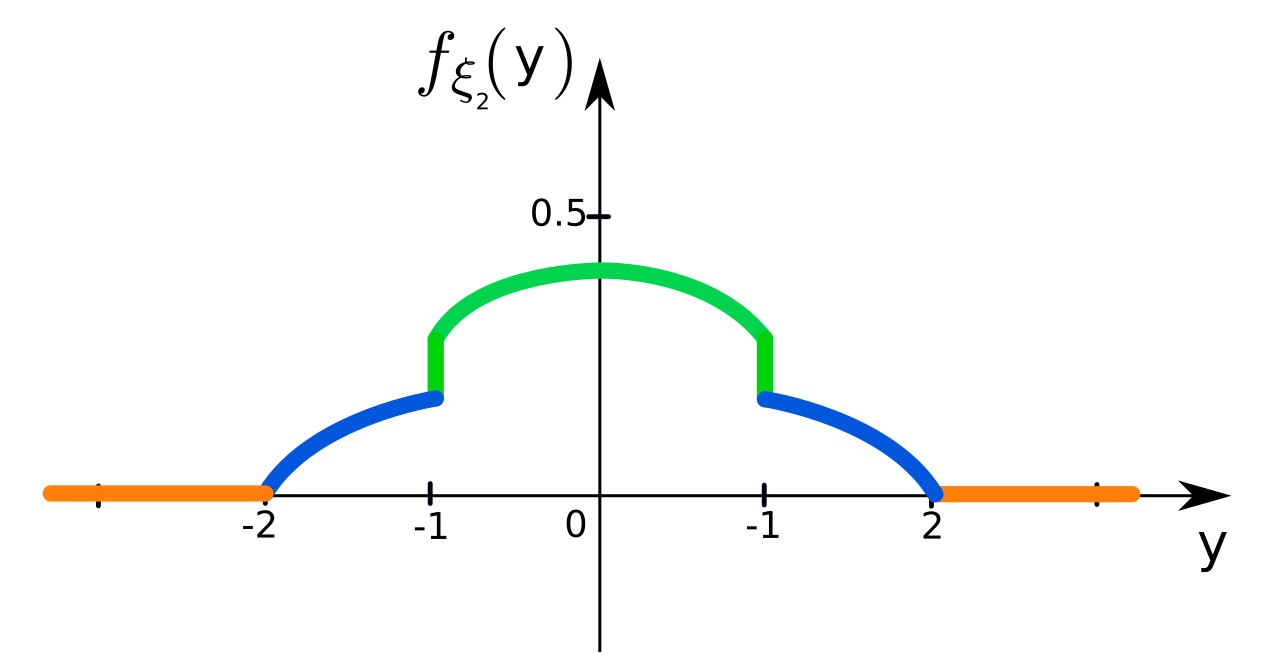
\includegraphics[scale=0.4]{assets/fxi21.png} \end{center}
Перевірка умови нормування:
$$
 \int\limits_{-\i}^{ +\infty}{ f_{\xi_2}(y)dy} = 0 + \frac{1}{ 2.5\pi + 2}
 \left( \int\limits_{-2}^{ -1}{ \sqrt{4 - y^2}dy }  +  \int\limits_{-1}^{ 1}{\left( \sqrt{4 - y^2} + \sqrt{1-y^2}+ 1  \right)dy} + \right.
$$
$$
+ \left. \int\limits_{-2}^{ -1}{ \sqrt{4 - y^2}dy } \right) =  \frac{1}{ 2.5\pi + 2}
\left( \int\limits_{-1}^{ 1}{dy}+  \int\limits_{-2}^{ 2}{\sqrt{4 - y^2}dy} +
 \int\limits_{-1}^{ 1}{\sqrt{1 - y^2} dy}
\right)=
$$
$$
= \left| \begin{gathered}
\text{Вже знаходили такі інтеграли за змінною } x \\
  \int\limits_{-1}^{ 1}{dy} = y\bigg|_{-1}^{1} = 2\\
	\int\limits_{-2}^{ 2}{\sqrt{4 - y^2}dy} =
	2\left( \frac{\sin{(2t)}}{2}   + t  \right)  \Bigg|_{ -\frac{\pi}{2} }^{ \frac{\pi}{2} 	} = 2 \pi \\
	 \int\limits_{-1}^{ 1}{\sqrt{1 - y^2}dy} = \frac{1}{2} \left(  \frac{\sin{(2t)}}{2}   + t  \right) \Bigg|^{ \frac{\pi}{2} }_{	-\frac{\pi}{2} 	} = \frac{\pi}{2}
\end{gathered} \right|
=(2 + \frac{\pi}{2} + 2\pi )\cdot \frac{1}{2 + 2.5\pi} = 1
$$

\newpage

\subsection{Функції розподілу координат $\xi_1$ та $\xi_2$.}
Нехай $F_{\xi_1}(x), F_{\xi_2}(y)$ функції розподілу координат вектора $\overline{\xi}$. Застосуємо формули:
$$
F_{\xi_1} (x) =  \int\limits_{-\i}^{ x}{f_{\xi_1}(t)dt}\qquad\quad
F_{\xi_2}(y) =  \int\limits_{-\i}^{ y}{ f_{\xi_2}(s)ds}
$$
\vfill
$$
F_{\xi_1} (x) = \begin{dcases}
0, \quad x \leq -1 ;\\
	  \int\limits_{-1}^{ x}\dfrac{2}{2.5\pi + 2} \sqrt{(1-s^2)}ds , \quad -1 < x \leq 0; \\
	\dfrac{2}{2.5\pi + 2} \left( \int\limits_{-1}^{ 0} \sqrt{(1-s^2)}ds +  \int\limits_{0}^{ x}{ds} \right)  , \quad 0 < x \leq 1; \\
	\dfrac{2}{2.5\pi + 2} \left( \int\limits_{-1}^{ 0} \sqrt{(1-s^2)}ds +  \int\limits_{0}^{ 1}{ds}  +  \int\limits_{1}^{ x}{\sqrt{4 - (s-1)^2}ds} \right)  , \quad 1 < x \leq 3; \\
	1, \quad x > 3 ;\\
\end{dcases}
$$
\vfill
$$
F_{\xi_1} (x) = \begin{cases}
0, \quad x \leq -1 ;\\
	  \frac{2}{2.5\pi + 2} \cdot \frac{ s\sqrt{1 - s^2} +\arcsin{\left( s  \right) }}{2}\Big|_{-1}^{x} , \quad -1 < x \leq 0; \\
	\frac{2}{2.5\pi + 2} \left( \frac{ s\sqrt{1 - s^2} +\arcsin{\left( s  \right) }}{2}\Big|_{-1}^{0} +  x \right)  , \quad 0 < x \leq 1; \\
	\frac{2}{2.5\pi + 2} \left( \frac{ s\sqrt{1 - s^2} +\arcsin{\left( s  \right) }}{2}\Big|_{-1}^{0} +  1 +
	\frac{ (s-1)\sqrt{4 - (s-1)^2} +4\arcsin{\left( \frac{s-1}{2}  \right) }}{2}\Big|_{1}^{x} \right)  , \quad 1 < x \leq 3; \\
	1, \quad x > 3 ;\\
\end{cases}
$$
\vfill
$$
F_{\xi_1} (x) = \begin{dcases}
0, \quad x \leq -1 ;\\
	  \dfrac{\arcsin\left(x\right)+x\sqrt{1-x^2}+\frac{{\pi}}{2} }{2.5\pi + 2} , \quad -1 < x \leq 0; \\
	\dfrac{\frac{{\pi}}{2} +  2x }{2.5\pi + 2} , \quad 0 < x \leq 1; \\
	\dfrac{\left(x-1\right)\sqrt{-x^2+2x+3}+4\arcsin\left(\frac{x-1}{2}\right) + \frac{\pi}{2}+2 }{2.5\pi + 2} , \quad 1 < x \leq 3; \\
	1, \quad x > 3 ;\\
\end{dcases}
$$
\vfill

\newpage
\vfill
Перевіримо на неперервність у точках стику:\\
$
 \lim\limits_{x\to  -1-}{ F_{\xi_1}(x)} =  \lim\limits_{x\to  1-}{ 0} =0
$\\
$
\lim\limits_{x\to  -1+}{ F_{\xi_1}(x)} =  \lim\limits_{x\to -1+}{\dfrac{\arcsin\left(x\right)+x\sqrt{1-x^2}+\frac{{\pi}}{2} }{2.5\pi + 2}} =
\dfrac{0- \frac{\pi}{2} +\frac{{\pi}}{2} }{2.5\pi + 2} = 0
$\\
$
\lim\limits_{x\to  0-}{ F_{\xi_1}(x)} = \lim\limits_{x\to 0-}{\dfrac{\arcsin\left(x\right)+x\sqrt{1-x^2}+\frac{{\pi}}{2} }{2.5\pi + 2}} = \dfrac{0+0+\frac{{\pi}}{2} }{2.5\pi + 2} = \dfrac{\pi}{5 \pi + 4}
$\\
$
\lim\limits_{x\to  -0+}{ F_{\xi_1}(x)} =  \lim\limits_{x\to  -0+}{\dfrac{\frac{{\pi}}{2} +  2x }{2.5\pi + 2}} = \dfrac{\frac{{\pi}}{2} + 0 }{2.5\pi + 2} = \dfrac{\pi}{5 \pi + 4}
$\\
$
\lim\limits_{x\to  1-}{ F_{\xi_1}(x)} =  \lim\limits_{x\to  1-}{\dfrac{\frac{{\pi}}{2} +  2x }{2.5\pi + 2}} =\dfrac{\frac{{\pi}}{2} +  2 }{2.5\pi + 2}
$\\
$
\lim\limits_{x\to  1+}{ F_{\xi_1}(x)} =  \lim\limits_{x\to 1+}{\dfrac{\left(x-1\right)\sqrt{-x^2+2x+3}+4\arcsin\left(\frac{x-1}{2}\right) + \frac{\pi}{2}+2 }{2.5\pi + 2} } =$\\$=  \dfrac{0\cdot\sqrt{-s^2+2s+3}-4\arcsin\left(0\right) + \frac{\pi}{2}+2 }{2.5\pi + 2}  = \dfrac{\frac{{\pi}}{2} +  2 }{2.5\pi + 2}
$\\
$\lim\limits_{x\to  3-}{ F_{\xi_1}(x)} =  \lim\limits_{x\to 3-}{\dfrac{\left(x-1\right)\sqrt{-x^2+2x+3}+4\arcsin\left(\frac{x-1}{2}\right) + \frac{\pi}{2}+2 }{2.5\pi + 2} } =$\\
$= \dfrac{2\sqrt{0}-4\arcsin\left(\frac{-4}{4}\right) + \frac{\pi}{2}+2 }{2.5\pi + 2} = \dfrac{0-4\cdot \left( -\frac{\pi}{2} \right)   + \frac{\pi}{2}+2 }{2.5\pi + 2} = 1$\\
$\lim\limits_{x\to  3+}{ F_{\xi_1}(x)} = \lim\limits_{x\to  3+}{1} = 1$
%  ІНТЕГРАЛ!!!
% $$
%  \int\limits_{}^{}{\sqrt{a^2 - t^2}dt}
% = a^2 \cdot \frac{ \frac{\sin{(2s)} }{2} +s}{2} +C =
% \frac{ t\sqrt{a^2 - t^2} +a^2\arcsin{\left( \frac{t}{a}  \right) }}{2} +C
% $$
\vfill
\begin{center}{\large Графік функції розподілу $F_{\xi_1}$}\\
 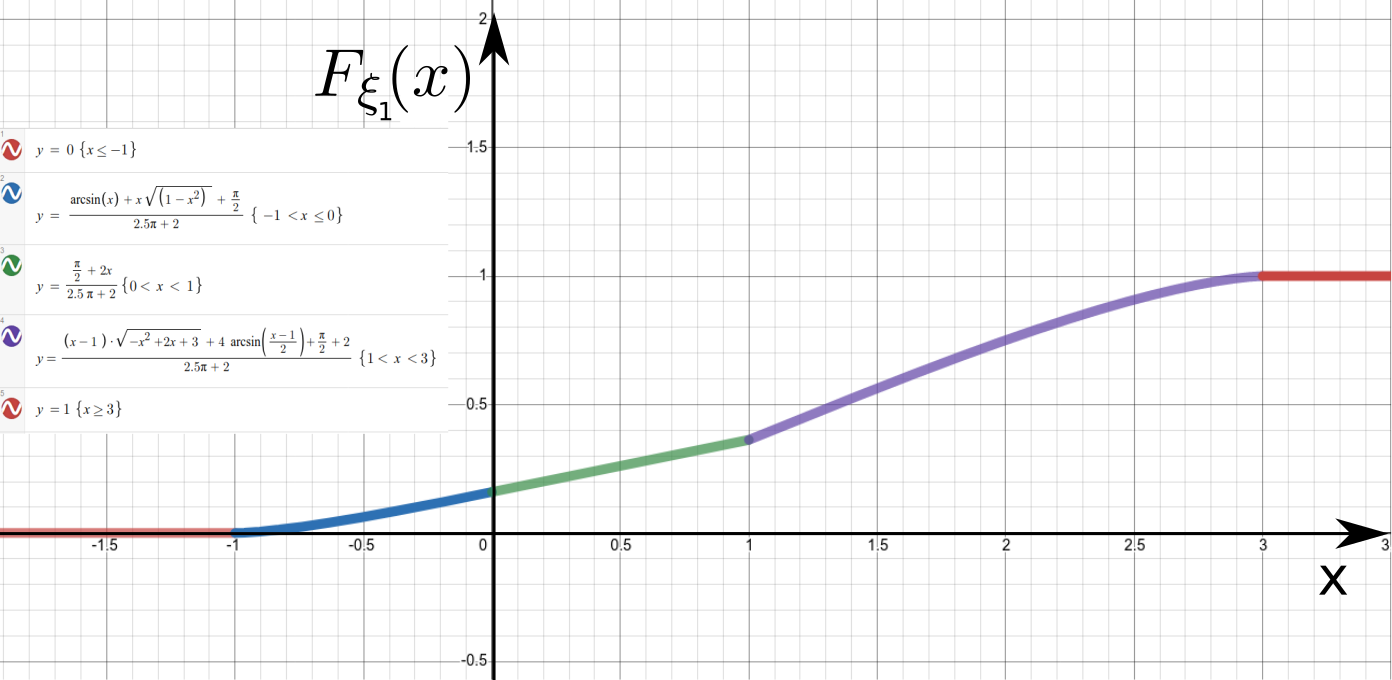
\includegraphics[scale=0.35]{assets/Fx22.png} \end{center}
 \vfill

$$
F_{\xi_2} (y) = \begin{dcases}
	0, \quad y \leq  -2;\\
	  \int\limits_{-2}^{ y}{ \dfrac{\sqrt{4 - s^2}}{2.5\pi + 2} ds}, \quad -2 < y \leq -1;\\
	\dfrac{1}{2.5\pi + 2} \cdot \left(\int\limits_{-2}^{ -1}{\sqrt{4 - s^2}  ds} + \int\limits_{-1}^{ y}{\sqrt{4 - s^2}+ \sqrt{1-s^2}+ 1 ds} \right),  -1 < y \leq 1; \\
			\dfrac{1}{2.5\pi + 2} \cdot \left(\int\limits_{-2}^{ -1}{\sqrt{4 - s^2}  ds} + \int\limits_{-1}^{ 1}{\left( \sqrt{4 - s^2}+ \sqrt{1-s^2}+ 1 ds \right) }\right. +\\+  \left. \int\limits_{1}^{ y}{\sqrt{4 - s^2}ds} \right), \quad 1 < y \leq 2;\\
			1, \quad y >  2;\\
\end{dcases}
$$
$$
F_{\xi_2} (y) = \begin{dcases}
	0, \quad y \leq  -2;\\
	 \dfrac{1}{2.5\pi + 2} \cdot \left( \dfrac{s\sqrt{4-s^2}}{2}+2\arcsin\left(\dfrac{s}{2}\right) \right)\Bigg|_{-2}^{y} , \quad -2 < y \leq -1;\\
	 \dfrac{1}{2.5\pi + 2} \left[ \cdot \left( \dfrac{s\sqrt{4-s^2}}{2}+2\arcsin\left(\dfrac{s}{2}\right) \right)\Bigg|_{-2}^{y} + \right.\\ \left. +\left( \dfrac{\arcsin\left(s\right)}{2}+\dfrac{s\sqrt{1-s^2}}{2}+s \right)\Bigg|_{-1}^{y}  \right] ,  -1 < y \leq 1; \\
	\dfrac{1}{2.5\pi + 2} \left[ \cdot \left( \dfrac{s\sqrt{4-s^2}}{2}+2\arcsin\left(\dfrac{s}{2}\right) \right)\Bigg|_{-2}^{y} + \right.\\ \left. +\left( \dfrac{\arcsin\left(s\right)}{2}+\dfrac{s\sqrt{1-s^2}}{2}+s \right)\Bigg|_{-1}^{1}  \right], \quad 1 < y \leq 2;\\
		1, \quad y >  2;\\
\end{dcases}
$$
$$
F_{\xi_2} (y) = \begin{dcases}
	0, \quad y \leq  -2;\\
	\dfrac{1}{2.5\pi + 2} \cdot \left( \dfrac{y\sqrt{4-y^2}+4\arcsin\left(\frac{y}{2}\right)}{2}+{\pi} \right) , \quad -2 < y \leq -1;\\
\dfrac{1}{2.5\pi + 2} \cdot \left( \dfrac{2\arcsin\left(y\right)+2y\sqrt{1-y^2}}{4} + \right. \\ \left. + \dfrac{y\sqrt{4-y^2}+4\arcsin\left(\frac{y}{2}\right)}{2}+1.25{\pi} + y + 1 \right) ,  -1 < y \leq 1; \\
		 	 \dfrac{1}{2.5\pi + 2} \cdot \left( \dfrac{{\pi}+4}{2} + \dfrac{y\sqrt{4-y^2}+4\arcsin\left(\frac{y}{2}\right)}{2}+{\pi} \right) , \quad 1 < y \leq 2;\\
		1, \quad y >  2;\\
\end{dcases}
$$

Перевіримо на неперервність у точках стику:\\
$
 \lim\limits_{y\to  -2-}{ F_{\xi_2}(y)} =  \lim\limits_{y\to  -2-}{0} = 0
$\\
$
 \lim\limits_{y\to  -2+}{ F_{\xi_2}(y)} =  \lim\limits_{y\to  -2+}{\dfrac{y\sqrt{4-y^2}+4\arcsin\left(\frac{y}{2}\right) + 2\pi}{5\pi + 4}} = \dfrac{
 -2*0+4 \frac{\pi}{2} +2{\pi}
 }{ 5\pi + 4}= 0
$\\
$
 \lim\limits_{y\to  -1-}{ F_{\xi_2}(y)} =  \lim\limits_{y\to  -1-}{\dfrac{y\sqrt{4-y^2}+4\arcsin\left(\frac{y}{2}\right) + 2\pi}{5\pi + 4}} = \dfrac{
 -\sqrt{3}-4 \frac{\pi}{6} +2{\pi}
 }{ 5\pi + 4} = \dfrac{-\sqrt{3} + \dfrac{4\pi}{3} }{5\pi + 4}
$\\
$
 \lim\limits_{y\to  -1+}{ F_{\xi_2}(y)} =  \lim\limits_{y\to  -1+}{\dfrac{1}{2.5\pi +
 2} \cdot \left( \dfrac{2\arcsin\left(y\right)+2y\sqrt{1-y^2}}{4} \right.}+$\\$+ \left. \dfrac{y\sqrt{4-y^2}+4\arcsin\left(\frac{y}{2}\right)}{2}+1.25{\pi} + y + 1 \right)  = \dfrac{- \dfrac{\pi}{2} -1 \cdot 0 - 	1\cdot \sqrt{3} - 4  \frac{\pi}{6} + 2.5\pi}{5\pi + 4}  =$\\$ = \dfrac{-\sqrt{3} + \dfrac{4\pi}{3} }{5\pi + 4}
$\\
$
\lim\limits_{y\to  1-}{ F_{\xi_2}(y)} =  \lim\limits_{y\to  1-}{\dfrac{1}{2.5\pi +
2} \cdot \left( \dfrac{2\arcsin\left(y\right)+2y\sqrt{1-y^2}}{4} \right.}+$\\$+ \left. \dfrac{y\sqrt{4-y^2}+4\arcsin\left(\frac{y}{2}\right)}{2}+1.25{\pi} + y + 1 \right)  = \dfrac{ \frac{\pi}{2} + 1\cdot 0 + \sqrt{3} + \frac{4\pi}{6} + 2.5\pi + 4  }{5\pi + 4} =
$\\
$
= \dfrac{ \sqrt{3} + \frac{11\pi}{3}  + 4  }{5\pi + 4}
$\\
$
\lim\limits_{y\to  1+ }{ F_{\xi_2}(y)} =  \lim\limits_{y\to 1+}{ \dfrac{1}{2.5\pi + 2} \cdot \left( \dfrac{{\pi}+4}{2} + \dfrac{y\sqrt{4-y^2}+4\arcsin\left(\frac{y}{2}\right)}{2}+{\pi} \right) } =
$\\
$
=\dfrac{1}{2.5\pi + 2} \cdot \dfrac{ \pi + 4}{ 2} + \frac{\sqrt{3} + \frac{4\pi}{6}  + 2\pi}{2} = \dfrac{ \sqrt{3} + \frac{11\pi}{3}  + 4  }{5\pi + 4}
$\\
$
\lim\limits_{y\to  2-}{ F_{\xi_2}(y)} =  \lim\limits_{y\to 2-}{ \dfrac{1}{2.5\pi + 2} \cdot \left( \dfrac{{\pi}+4}{2} + \dfrac{y\sqrt{4-y^2}+4\arcsin\left(\frac{y}{2}\right)}{2}+{\pi} \right) } =
$
$
= \dfrac{1}{2.5\pi + 2} \cdot\dfrac{\pi + 4 + 2\cdot 0 + \frac{4\pi}{2} + 2\pi }{2} = \dfrac{5\pi + 4}{4\pi + 4} = 1
$\\
$\lim\limits_{y\to  2+}{ F_{\xi_2}(y)} = 1$\\
Тож, знайдені функції розподілу $F_{\xi_1}(x), F_{\xi_2}(y)$ задовольняють умові неперервності. Але, можемо дещо спростити $ F_{\xi_2}(y)$ виконавши алгебраічні перетворення:
\vfill
$$
F_{\xi_2} (y) = \begin{dcases}
	0, \quad y \leq  -2;\\
 \dfrac{y\sqrt{4-y^2}+4\arcsin\left(\frac{y}{2}\right) + 2{\pi}}{10\pi + 4} , \quad -2 < y \leq -1;\\
 \dfrac{\arcsin\left(y\right)+y\sqrt{1-y^2}+ y\sqrt{4-y^2}+4\arcsin\left(\frac{y}{2}\right) + 2.5\pi + 2y + 2}{5\pi + 4}   ,\\  -1 < y \leq 1; \\
		 	 \dfrac{3\pi + 4 +y\sqrt{4-y^2}+4\arcsin\left(\frac{y}{2}\right)}{5\pi + 4} , \quad 1 < y \leq 2;\\
		1, \quad y >  2;\\
\end{dcases}
$$
\vfill
\begin{center}{\large Графік функції розподілу $F_{\xi_2}$}\\
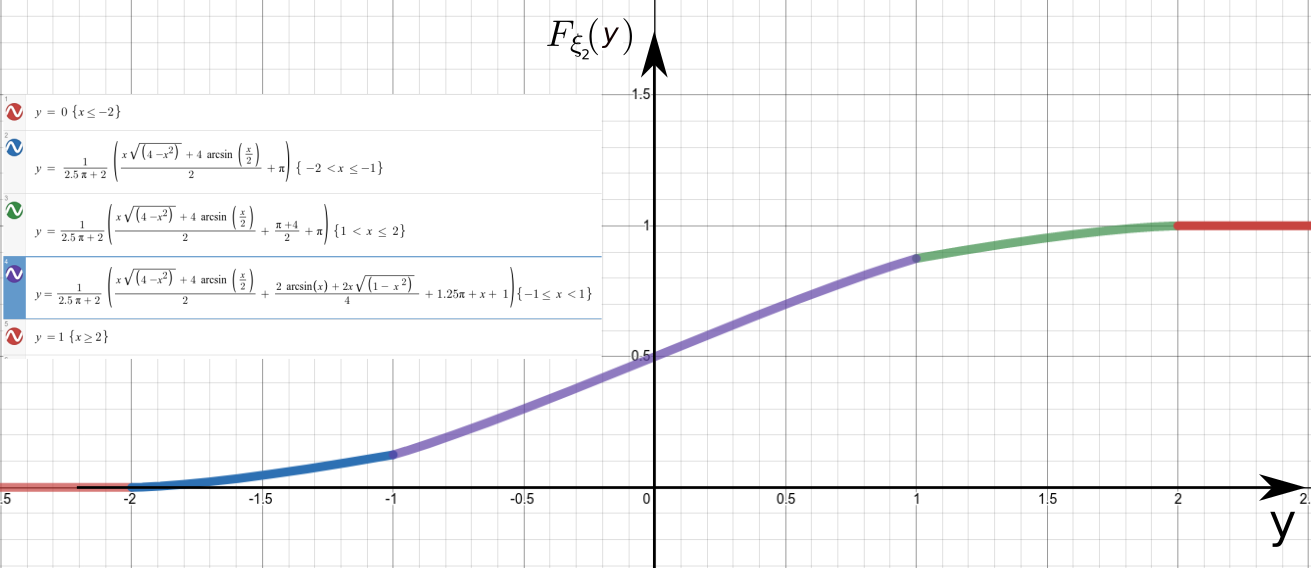
\includegraphics[scale=0.4]{assets/Fx4556.png} \end{center}

\newpage

\subsection{Сумісна функція розподілу випадкового вектора $\overline{\xi}$
}
Згідно означення $F_{\overline{\xi}}(x,y) = \mathbb{P} \left\lbrace \xi_1 < x, \xi_2 < y \right\rbrace$.
Скористаємося формулою:
$$
\Fx (x,y )  =  \int\limits_{-\i}^{ x}{ dt  \int\limits_{-\i}^{ y}{ \fx (t,s) ds}}
$$

Координатну площину $XOY$ розіб’ємо на області $D_1, D_2,..., D_{14}$.

\begin{center} 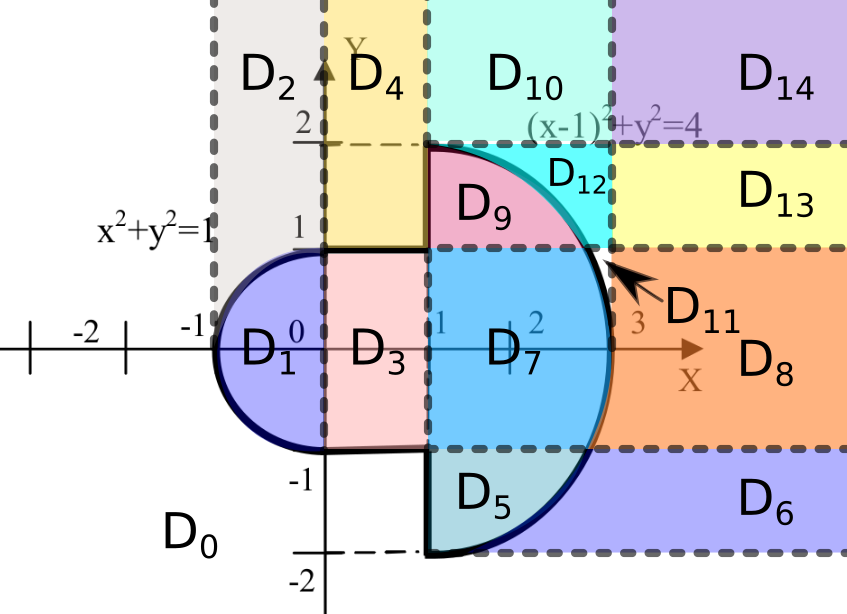
\includegraphics[scale=0.35]{assets/fixobl0.png}
\end{center}
1. $D_0 = \left\lbrace (x,y) \Bigg| \begin{gathered}
 (x\leq -1)  \lor \left( (x \leq  -\sqrt{1 - y^2}) \land (y \leq  -\sqrt{1-x^2}) \right) \lor \\
 \lor \left( (0 \leq x \leq 1 )\land ( -2  \leq y \leq -1) \right) \lor (y \leq -2)
\end{gathered} \right\rbrace $\\
2. $D_1 = \left\lbrace (x,y) \big| \begin{gathered}
(x\leq 0) \land (x^2 + y^2 < 1)
\end{gathered} \right\rbrace $\\
3.  $D_2 = \left\lbrace (x,y) \big| \begin{gathered}
\left( (-1<x\leq 0) \land (1<y) \right)
\lor \left( (x \leq  -\sqrt{1 - y^2}) \land (y \geq   \sqrt{1-x^2}) \right)
\end{gathered} \right\rbrace $\\
4.  $D_3 = \left\lbrace (x,y) \big| \begin{gathered}
( 0 < x \leq 1) \land (-1 < y \leq 1)
\end{gathered} \right\rbrace $\\
5. $D_4 = \left\lbrace (x,y) \big| \begin{gathered}
( 0 < x \leq 1) \land (1 < y )
\end{gathered} \right\rbrace $\\
6. $D_5 = \left\lbrace (x,y) \big| \begin{gathered}
\left( (x-1)^2 + y^2 < 2 \right) \land ( y \leq -1 ) \land (x >1)
\end{gathered} \right\rbrace $\\
7. $D_6 = \left\lbrace (x,y) \big| \begin{gathered}
(-2 < y \leq  -1) \land \left( (x-1)^2 + y^2 \geq 2 \right) \land (x > 1)
\end{gathered} \right\rbrace $\\
8. $D_7 = \left\lbrace (x,y) \big| \begin{gathered}
\left( (x-1)^2 + y^2 < 2 \right) \land (-1< y \leq 1 ) \land (x >1)
\end{gathered} \right\rbrace $\\
9. $D_8 = \left\lbrace (x,y) \big| \begin{gathered}
\left( (-1 < y \leq  0) \land \left( (x-1)^2 + y^2 \geq 2 \right) \land (x > 1) \right) \\ \lor
\left( (3 < x ) \land (0 <y \leq 1)  \right)
\end{gathered} \right\rbrace $\\
10. $D_9 = \left\lbrace (x,y) \big| \begin{gathered}
(1 < y \leq  2) \land \left( (x-1)^2 + y^2 \geq 2 \right) \land (x > 1)
\end{gathered} \right\rbrace $\\
11. $D_{10} = \left\lbrace (x,y) \big| \begin{gathered}
( 1 < x \leq 3) \land (2 < y )
\end{gathered} \right\rbrace $\\
12. $D_{11} = \left\lbrace (x,y) \big| \begin{gathered}
(0 < y \leq  1) \land \left( (x-1)^2 + y^2 \geq 2 \right) \land (0 < x \leq 3)
\end{gathered} \right\rbrace $\\
13. $D_{12} = \left\lbrace (x,y) \big| \begin{gathered}
(1 < y \leq  2) \land \left( (x-1)^2 + y^2 \geq 2 \right) \land (0 < x \leq 3)
\end{gathered} \right\rbrace $\\
14. $D_{13} = \left\lbrace (x,y) \big| \begin{gathered}
\left( (3 < x ) \land (1 <y \leq 2)  \right)
\end{gathered} \right\rbrace $\\
15. $D_{14} = \left\lbrace (x,y) \big| \begin{gathered}
\left( (3 < x ) \land (2<y)  \right)
\end{gathered} \right\rbrace $\\

\newpage

1. $(x,y) \in D_0$
\begin{center} 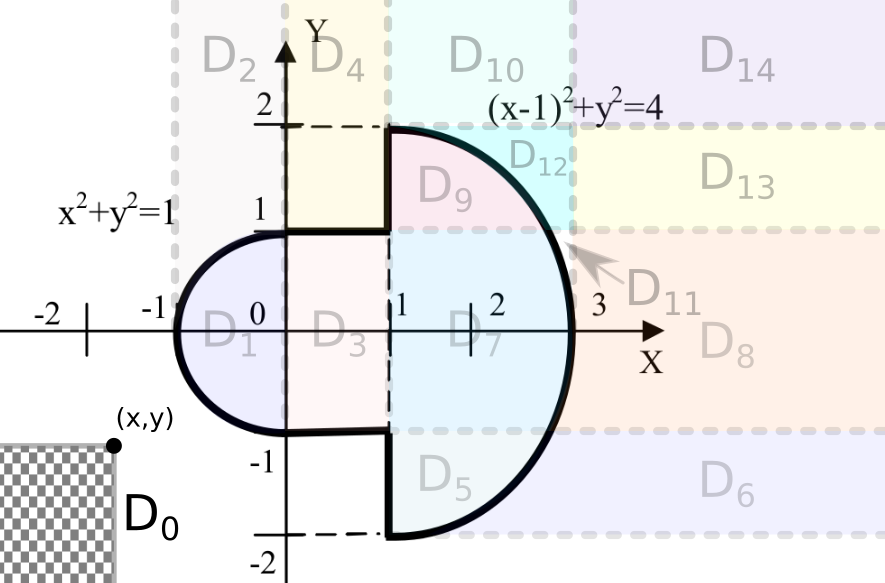
\includegraphics[scale=0.4]{assets/zone10.png} \end{center}
$$
\Fx (x,y) = 0
$$
Перевірка:
$\dfrac{\d^2 \Fx}{\d x \d y}(x,y) = 0  = \fx (x,y)$
\newpage

2. $(x,y) \in D_1$
\begin{center} 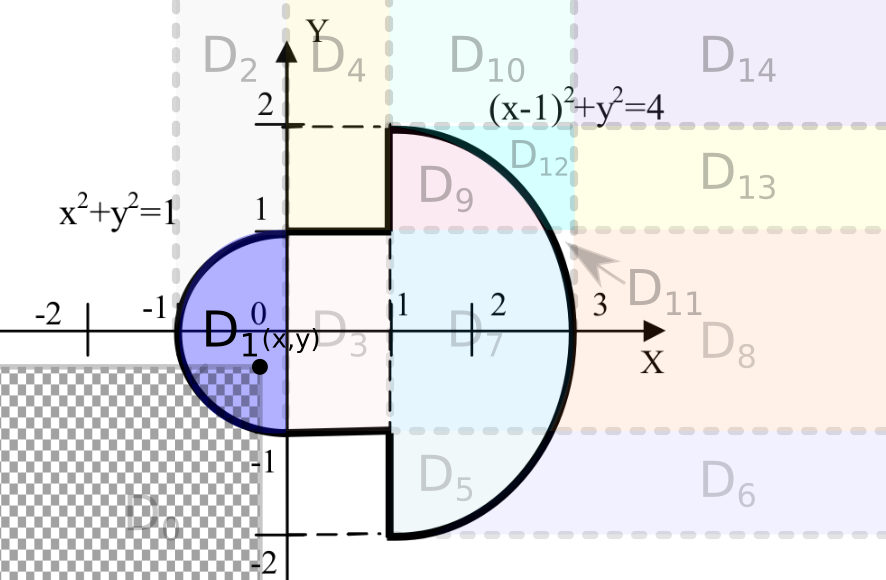
\includegraphics[scale=0.4]{assets/zone21.png} \end{center}
$$
\Fx (x,y) =  \frac{1}{2.5\pi + 2} \cdot  \int\limits_{-\sqrt{1- x^2}}^{y}{ds  \int\limits_{-\sqrt{1-s^2}}^{x}{dt}} =   \int\limits_{-\sqrt{1- x^2}}^{y}{x+\sqrt{1-s^2}ds  } =
$$
$$
=\frac{1}{2.5\pi + 2} \cdot \dfrac{\arcsin\left(y\right)+y\sqrt{1-y^2}+2xy+\arcsin\left(\sqrt{1-x^2}\right)+3x\sqrt{1-x^2}}{2}
$$
Перевірка:\\
$\dfrac{\d^2 \Fx}{\d x \d y}(x,y) = \dfrac{\d^2}{\d x \d y} \left( \dfrac{\arcsin\left(y\right)+y\sqrt{1-y^2}+2xy+\arcsin\left(\sqrt{1-x^2}\right)+3x\sqrt{1-x^2}}{5\pi + 4}  \right) =$\\
$ = \frac{1}{2.5\pi + 2} \cdot \dfrac{\d}{\d x} \left( \dfrac{x\sqrt{1-y^2}-y^2+1}{\sqrt{1-y^2}} \right) =\frac{1}{2.5\pi + 2} \cdot 1  =\fx (x,y)$\\
Перевірка ліній стику областей:\\
$D_0 - D_1: y = -\sqrt{1- x^2}, (y \leq 0)$\\
$ \Fx (x,-\sqrt{1- x^2})^{D_1} = $\\
$=\dfrac{\arcsin\left(-\sqrt{1-x^2}\right)-x\sqrt{1-x^2}-2x\sqrt{1-x^2}+\arcsin\left(\sqrt{1-x^2}\right)+3x\sqrt{1-x^2}}{5\pi + 4} =$
\\$= 0= \Fx (x,-\sqrt{1- x^2})^{D_0} = 0$
\newpage
3. $(x,y) \in D_2$
\begin{center} 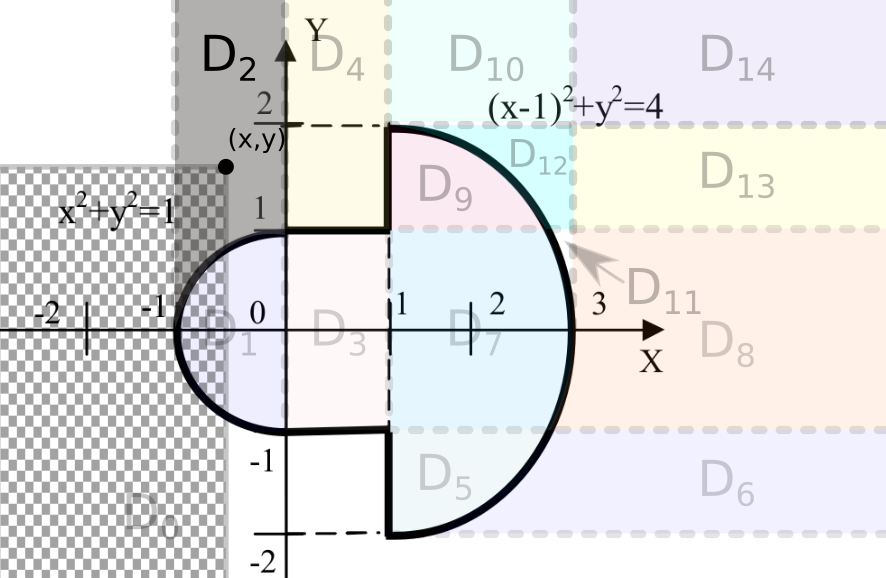
\includegraphics[scale=0.4]{assets/zone32.png} \end{center}
$$
\Fx (x,y) =  \frac{1}{2.5\pi + 2} \cdot  \int\limits_{-\sqrt{1- x^2}}^{\sqrt{1- x^2}}{ds  \int\limits_{-\sqrt{1-s^2}}^{x}{dt}} =
\frac{1}{2.5\pi + 2} \cdot  \int\limits_{-\sqrt{1- x^2}}^{\sqrt{1- x^2}}{\sqrt{1-s^2}+xds  }
$$
$$
= \frac{1}{2.5\pi + 2} \cdot \left( \arcsin\left(\sqrt{1-x^2}\right)+x\sqrt{1-x^2} \right)
$$
Перевірка:\\
$\dfrac{\d^2 \Fx}{\d x \d y}(x,y) = \dfrac{\d^2}{\d x \d y} \left( \frac{1}{2.5\pi + 2} \cdot\arcsin\left(\sqrt{1-x^2}\right)+x\sqrt{1-x^2} \right) =$\\
$ = \frac{1}{2.5\pi + 2} \cdot \dfrac{\d}{\d x} 0 = 0 =\fx (x,y)$\\

Перевірка ліній стику областей:\\
$D_1 - D_2: y = \sqrt{1- x^2}$\\
$ \Fx (x,\sqrt{1- x^2})^{D_1} = $\\
$=\dfrac{\arcsin\left(\sqrt{1-x^2}\right)-x\sqrt{1-x^2}+2x\sqrt{1-x^2}+\arcsin\left(\sqrt{1-x^2}\right)+x\sqrt{1-x^2}}{5\pi + 4} =$
\\$= \frac{1}{2.5\pi + 2} \cdot \left( \arcsin\left(\sqrt{1-x^2}\right)+x\sqrt{1-x^2} \right)  =\Fx (x,-\sqrt{1+x^2})^{D_2}$
\newpage
4. $(x,y) \in D_3$
\begin{center} 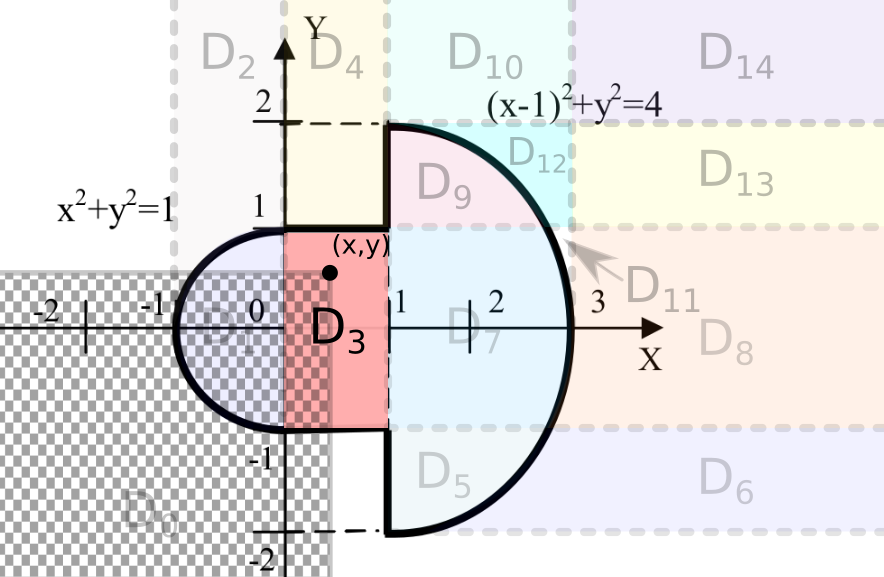
\includegraphics[scale=0.4]{assets/zone43.png} \end{center}
$$
\Fx (x,y) =  \Fx (0,y)^{D_1}+ \frac{1}{2.5\pi + 2} \cdot  \int\limits_{0}^{ x}{dt  \int\limits_{-1}^{y }{ds}} =$$\\$$= \frac{1}{2.5\pi + 2} \cdot \left( \dfrac{\arcsin\left(y\right)+y\sqrt{1-y^2} + \frac{\pi}{2} }{2}+ x(y+1)\right)
$$

Перевірка:\\
$\dfrac{\d^2 \Fx}{\d x \d y}(x,y) = \dfrac{\d^2}{\d x \d y} \left(\frac{1}{2.5\pi + 2} \cdot \left( \dfrac{\arcsin\left(y\right)+y\sqrt{1-y^2} + \frac{\pi}{2} }{2}+ x(y+1)\right) \right) =$\\
$ = \frac{1}{2.5\pi + 2} \cdot \dfrac{\d}{\d y} (y+1) = \frac{1}{2.5\pi + 2} =\fx (x,y)$\\

Перевірка ліній стику областей:\\
$D_2 - D_3: x = 0$\\
$ \Fx (0,y)^{D_1} =\frac{1}{2.5\pi + 2} \cdot\dfrac{\arcsin\left(y\right)+y\sqrt{1-y^2} + \frac{\pi}{2} }{2} =\Fx (0,y)^{D_3}$

\newpage
5. $(x,y) \in D_4$
\begin{center} 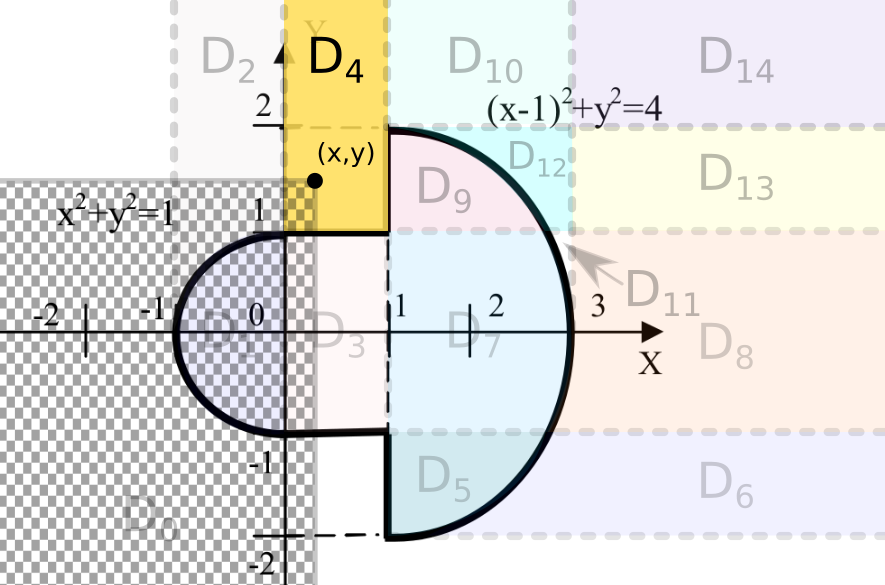
\includegraphics[scale=0.4]{assets/zone655.png} \end{center}
$$
\Fx (x,y) =  \Fx (x, 1)^{D_3} = \frac{1}{2.5\pi + 2} \cdot \left( \dfrac{\pi}{2}+ 2x\right)
$$

Перевірка:\\
$\dfrac{\d^2 \Fx}{\d x \d y}(x,y) =
\dfrac{\d^2}{\d x \d y} \left( \frac{1}{2.5\pi + 2} \cdot \left( \dfrac{\pi}{2}+ 2x\right)
\right) = 0 =\fx (x,y)$\\

Перевірка ліній стику областей:\\
$D_2 - D_4: x = 0$\\
$ \Fx (0,y)^{D_2} =\frac{\arcsin(1)}{2.5\pi + 2}   = \frac{\pi}{5\pi + 4} = \Fx (0,y)^{D_3}$\\
\newpage

6. $(x,y) \in D_5$
\begin{center} 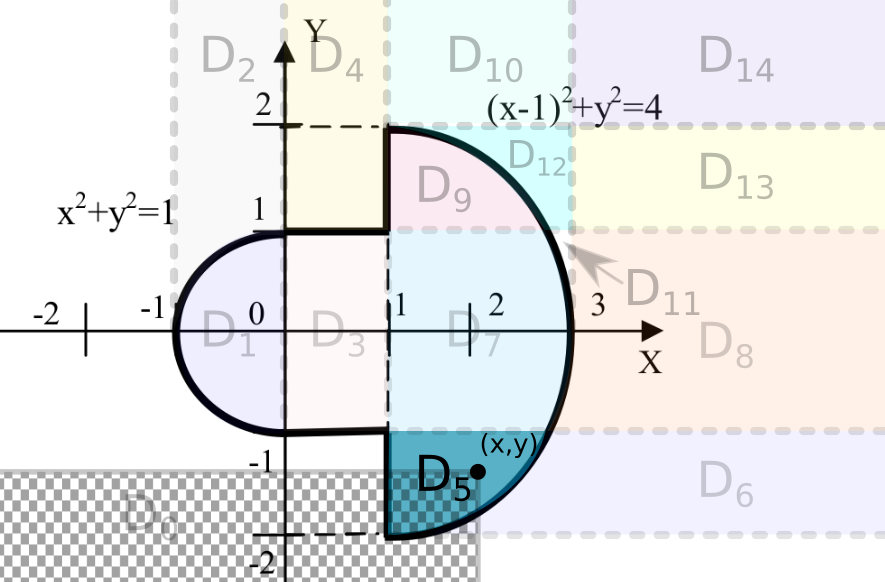
\includegraphics[scale=0.4]{assets/zone54.png} \end{center}
$$
\Fx (x,y) = \frac{1}{2.5\pi + 2} \cdot \int\limits_{1}^{x}{dt  \int\limits_{-\sqrt{4 - (t-1)^2}}^{ y}{ds}}   = \frac{1}{2.5\pi + 2} \cdot  \int\limits_{1}^{x}{\sqrt{4-\left(t-1\right)^2}+y dt}  =
$$
$$
=\frac{1}{2.5\pi + 2} \cdot \dfrac{\left(2x-2\right)y+\left(x-1\right)\sqrt{-x^2+2x+3}+4\arcsin\left(\frac{x-1}{2}\right)}{2}
$$

Перевірка:\\
$\dfrac{\d^2 \Fx}{\d x \d y}(x,y) =
\dfrac{\d^2}{\d x \d y} \left( \dfrac{\left(2x-2\right)y+\left(x-1\right)\sqrt{-x^2+2x+3}+4\arcsin\left(\frac{x-1}{2}\right)}{5\pi + 4}\right) = $\\$=\dfrac{1}{2.5\pi + 2} \cdot  \dfrac{\d}{\d x} \dfrac{2x-2}{2} = \dfrac{1}{2.5\pi + 2}  =\fx (x,y)$\\

Перевірка ліній стику областей:\\
$D_0 - D_5: x = 1$\\
$ \Fx (1,y)^{D_0} = 0 =  \Fx (1,y)^{D_3} = \frac{0*y + 0\sqrt{3} + 4* 0}{5\pi + 4} =  0$\\
\newpage

7. $(x,y) \in D_6$
\begin{center} 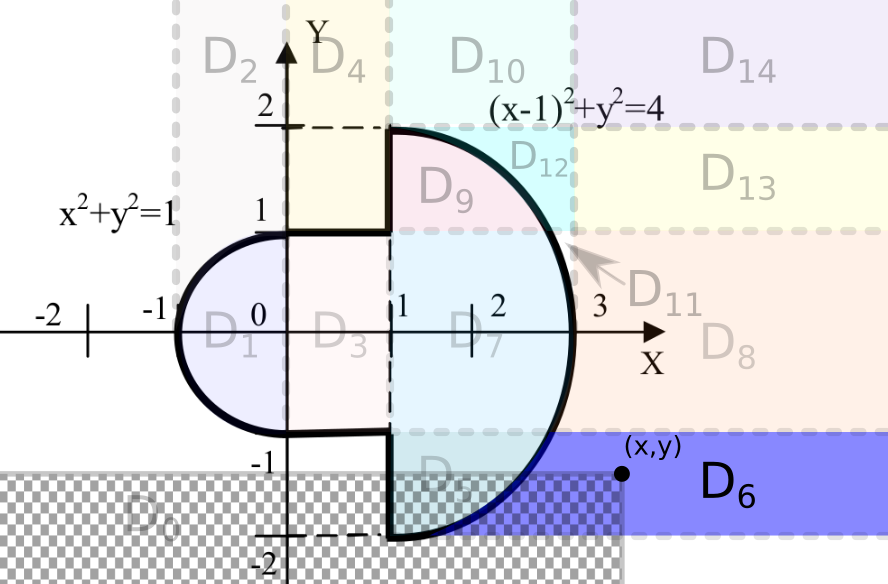
\includegraphics[scale=0.4]{assets/zone766.png} \end{center}
$$
\Fx (x,y) =  \Fx (1+\sqrt{4 - y^2}, y)^{D_5} =  \dfrac{2\left(y\sqrt{4 - y^2}\right)-y\sqrt{4 - y^2}+4\arcsin\left(\frac{\sqrt{4 - y^2}}{2}\right)}{5\pi +4}=
$$
$$
= \dfrac{\left(y\sqrt{4 - y^2}\right) + 4\arcsin\left(\frac{\sqrt{4 - y^2}}{2}\right)}{5\pi +4} =  \dfrac{y\sqrt{4 - y^2} + 4\arcsin\left(\dfrac{y}{2}\right) + 2\pi }{5\pi +4}
$$


Перевірка:\\
$\dfrac{\d^2 \Fx}{\d x \d y}(x,y) =
\dfrac{\d^2}{\d x \d y} \left(  \dfrac{y\sqrt{4 - y^2} + 4\arcsin\left(\dfrac{y}{2}\right) + 2\pi }{5\pi +4}
\right) = \dfrac{\d}{ \d y} \left(0 \right)  = 0=\fx (x,y)$\\

Перевірка ліній стику областей:\\
$D_6 - D_5: x = 1 + \sqrt{4 - y^2}$\\
$ \Fx (1 + \sqrt{4 - y^2},y)^{D_5} =  \dfrac{y\sqrt{4 - y^2} + 4\arcsin\left(\dfrac{y}{2}\right) + 2\pi }{5\pi +4} = \Fx (1 + \sqrt{4 - y^2},y)^{D_6}$\\
$D_6 - D_0: y = -2$\\
$ \Fx (x,-2)^{D_5} =  \frac{0\cdot (-2) + 4 \cdot \frac{-\pi}{2}+ 2\pi  }{5\pi +4} = 0  = \Fx (x,-2)^{D_0} = 0$\\

\newpage

8. $(x,y) \in D_7$
\begin{center} 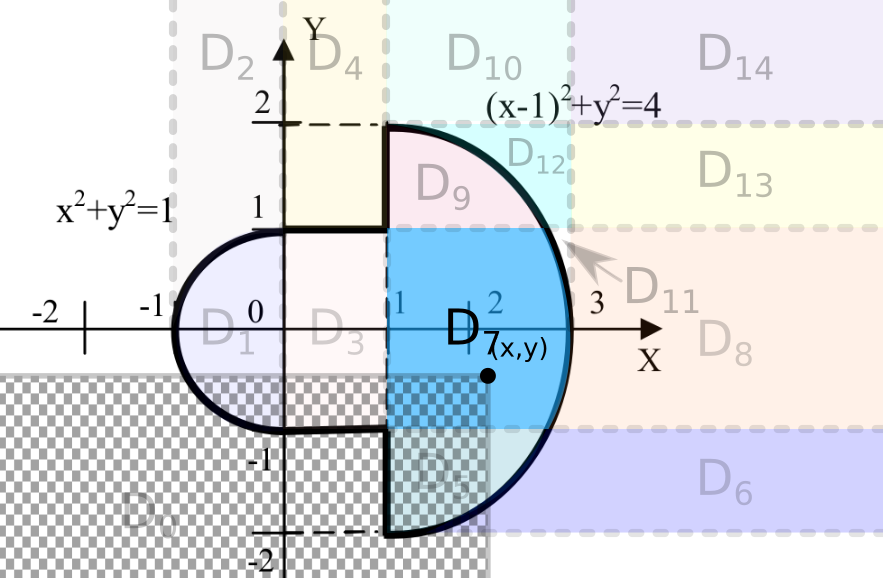
\includegraphics[scale=0.3]{assets/zone885.png} \end{center}
$$
\Fx (x,y) =  \Fx (1, y)^{D_3} + \Fx (x, -1)^{D_5} +\frac{1}{2.5\pi + 2} \cdot  \int\limits_{1}^{ x}{ds  \int\limits_{-1}^{ y}{ dt}} =
$$
$$
= \frac{1}{2.5\pi + 2} \cdot \left( \dfrac{\arcsin\left(y\right)+y\sqrt{1-y^2} + \frac{\pi}{2} }{2}+ (y+1) \right.+$$\\$$+\left. \dfrac{\left(2-2x\right)+\left(x-1\right)\sqrt{-x^2+2x+3}+4\arcsin\left(\frac{x-1}{2}\right)}{2} + (x-1)(y+1)\right)=
$$
$
=\frac{\arcsin\left(y\right)+y\sqrt{1-y^2} + \frac{\pi}{2} + \left(2-2x\right)+\left(x-1\right)\sqrt{-x^2+2x+3}+4\arcsin\left(\frac{x-1}{2}\right)+ 2x(y+1)}{5\pi + 4}
$

Перевірка:\\
$\dfrac{\d^2 \Fx}{\d x \d y}(x,y) =
\dfrac{\d^2}{\d x \d y} \left(  \frac{\arcsin\left(y\right)+y\sqrt{1-y^2} + \frac{\pi}{2} + \left(2-2x\right)+\left(x-1\right)\sqrt{-x^2+2x+3}+4\arcsin\left(\frac{x-1}{2}\right)+ 2x(y+1)}{5\pi + 4}
\right) =$\\
$= \dfrac{\d}{ \d x} {\dfrac{\left(x\sqrt{1-y^2}-y^2+1\right)}{(2.5\pi + 2)\sqrt{1-y^2}}} = \frac{1}{2.5\pi + 2}=\fx (x,y)$\\

Перевірка ліній стику областей:\\
$D_7 - D_5: y = -1$\\
$ \Fx (x,-1)^{D_7} =  \frac{0+0 + \left(2-2x\right)+\left(x-1\right)\sqrt{-x^2+2x+3}+4\arcsin\left(\frac{x-1}{2}\right)+0}{5\pi + 4} =$\\$= \Fx (x,-1)^{D_5}= \frac{1}{2.5\pi + 2} \cdot \frac{\left(2-2x\right)+\left(x-1\right)\sqrt{-x^2+2x+3}+4\arcsin\left(\frac{x-1}{2}\right)}{2} = $\\
$D_7 - D_3 : x = 1$\\
$ \Fx (1,y)^{D_7} = \frac{\arcsin\left(y\right)+y\sqrt{1-y^2} + \frac{\pi}{2} + 0+0+4\arcsin\left(\frac{x-1}{2}\right)+ 2(y+1)}{5\pi + 4} =$\\
$= \Fx (1,y)^{D_3} = \frac{1}{2.5\pi + 2} \cdot \left( \frac{\arcsin\left(y\right)+y\sqrt{1-y^2} + \frac{\pi}{2} }{2}+ (y+1)\right)$
\newpage

9. $(x,y) \in D_{13}$
\begin{center} 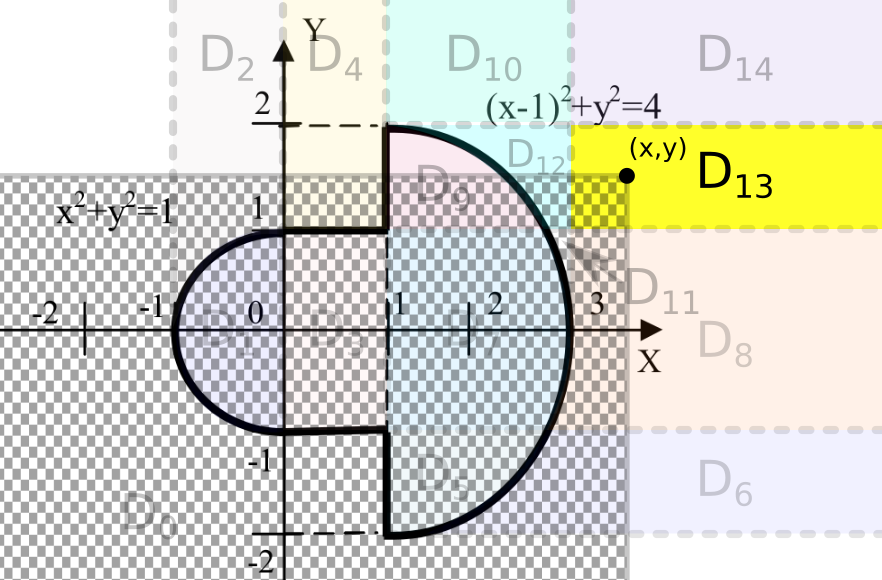
\includegraphics[scale=0.4]{assets/zone131245.png} \end{center}
$$
\Fx (x,y) =1 -  \frac{1}{2.5\pi + 2} \cdot  \int\limits_{y}^{ 2}{dt  \int\limits_{1}^{1 + \sqrt{4 - t^2}}{ds}}  =\dfrac{3\pi + 4 + y\sqrt{4-y^2}+4\arcsin\left(\frac{y}{2} \right)}{5\pi + 4}
$$

Перевірка:\\
$\dfrac{\d^2 \Fx}{\d x \d y}(x,y) =
\dfrac{\d^2}{\d x \d y} \left( \dfrac{3\pi + 4 + y\sqrt{4-y^2}+4\arcsin\left(\frac{y}{2} \right)}{5\pi + 4} \right)  = \frac{\d}{\d y}0 = 0=\fx (x,y)$\\

Перевірка ліній стику областей:\\
Зробимо пізніше, коли знайдемо функції розподілу у інших зонах.
\newpage

10. $(x,y) \in D_9$
\begin{center} 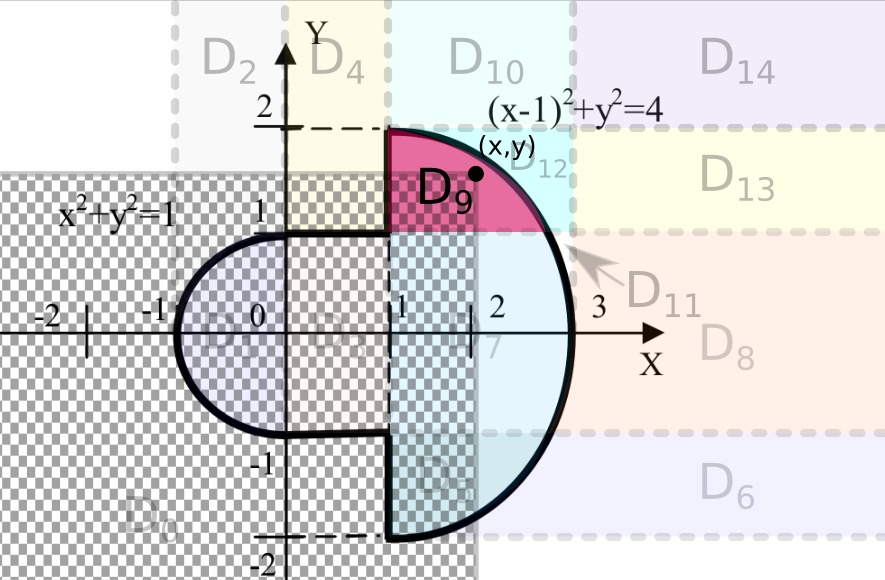
\includegraphics[scale=0.4]{assets/zone1091.png} \end{center}
$$
\Fx (x,y) =  \Fx (x, 1)^{D_7} + \frac{1}{2.5\pi + 2} \cdot  \int\limits_{1}^{ x}{ds  \int\limits_{1}^{ y}{dt}} =
$$
\begin{center}
$
=\frac{\left(2-2x\right)+\left(x-1\right)\sqrt{-x^2+2x+3}+4\arcsin\left(\frac{x-1}{2}\right)+ 4x +\pi}{5\pi + 4} + \frac{2(x-1)(y-1)}{5\pi + 4} =
$\\
$
=\frac{\left(x-1\right)\sqrt{-x^2+2x+3}+4\arcsin\left(\frac{x-1}{2}\right)+4 +2y(x-1) +\pi}{5\pi + 4}
$
\end{center}


Перевірка:\\
$\dfrac{\d^2 \Fx}{\d x \d y}(x,y) =
\dfrac{\d^2}{\d x \d y} \left( \frac{\left(x-1\right)\sqrt{-x^2+2x+3}+4\arcsin\left(\frac{x-1}{2}\right)+4 +2y(x-1) +\pi}{5\pi + 4}
\right) =$\\
$= \dfrac{\d}{ \d x} \dfrac{2x-2}{5\pi + 4} = \dfrac{1}{2.5\pi + 2}=\fx (x,y)$\\

Перевірка ліній стику областей:\\
$D_9 - D_7: y = 1$\\
$ \Fx (x,1)^{D_9} =  \frac{\left(x-1\right)\sqrt{-x^2+2x+3}+4\arcsin\left(\frac{x-1}{2}\right)+4 +2(x-1) +\pi}{5\pi + 4} =$\\
$ \Fx (x,1)^{D_7} = \frac{\pi+ 0 + 2-2x+\left(x-1\right)\sqrt{-x^2+2x+3}+4\arcsin\left(\frac{x-1}{2}\right)+ 4x}{5\pi + 4}$\\
$D_9 - D_4 : x = 1$\\
$ \Fx (1,y)^{D_9} = \frac{0+4\arcsin(0)+4 +\pi}{5\pi + 4} =$\\
$= \Fx (1,y)^{D_4} = \frac{1}{2.5\pi + 2} \cdot \left( \frac{\pi}{2} + 2 \right)$
\newpage

11. $(x,y) \in D_{10}$
\begin{center} 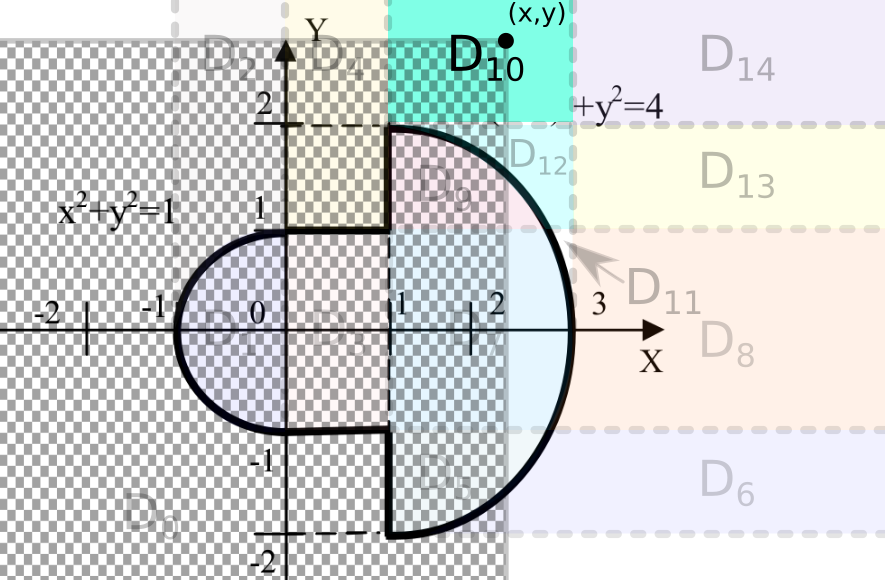
\includegraphics[scale=0.4]{assets/1110.png} \end{center}
$$
\Fx (x,y) =  1 -   \frac{1}{2.5\pi + 2} \cdot \int\limits_{x}^{ 3}{ dt  \int\limits_{\sqrt{4 - (t-1)^2}}^{ - \sqrt{4 - (t-1)^2}}{ds}}=   1 + \frac{2}{2.5\pi + 2} \cdot  \int\limits_{3}^{ x}{\sqrt{4 - (t-1)^2}dt} =
$$
$$
= \dfrac{\left(x-1\right)\sqrt{-x^2+2x+3}+4\arcsin\left(\frac{x-1}{2}\right)-2{\pi}}{2.5\pi + 2}+ 1  =
$$
$$
= \dfrac{\left(x-1\right)\sqrt{-x^2+2x+3}+4\arcsin\left(\frac{x-1}{2}\right) + \frac{\pi}{2} + 2 }{2.5\pi + 2}
$$

Перевірка:\\
$\dfrac{\d^2 \Fx}{\d x \d y}(x,y) =
\dfrac{\d^2}{\d x \d y} \left( \frac{\left(x-1\right)\sqrt{-x^2+2x+3}+4\arcsin\left(\frac{x-1}{2}\right)+\frac{{\pi}}{2}+2}{2.5\pi + 2}
\right) = \dfrac{\d}{ \d x} 0 = 0=\fx (x,y)$\\

Перевірка ліній стику областей:\\
$D_{10} - D_4 : x = 1$\\
$ \Fx (1,y)^{D_10} = \frac{0+4\arcsin(0)+4 +\pi/2 + 2}{2.5\pi + 2} = \frac{ \frac{\pi}{2} + 2  }{2.5\pi + 2}  = \Fx (x,y)^{D_4}$\\
\newpage



12. $(x,y) \in D_8$.
З малюнку та інтегралу видно, що зону $D_8$ доведеться розбити ще на 2: $-1<y \leq 0$ та $ 0< y < 1$, але функції розподілу виявилися однаковими. Для $-1<y \leq 0$ можемо скористатися вже знайденим виразом (при обчисленні виникає модуль, який розкриваємо з -):
\begin{center} 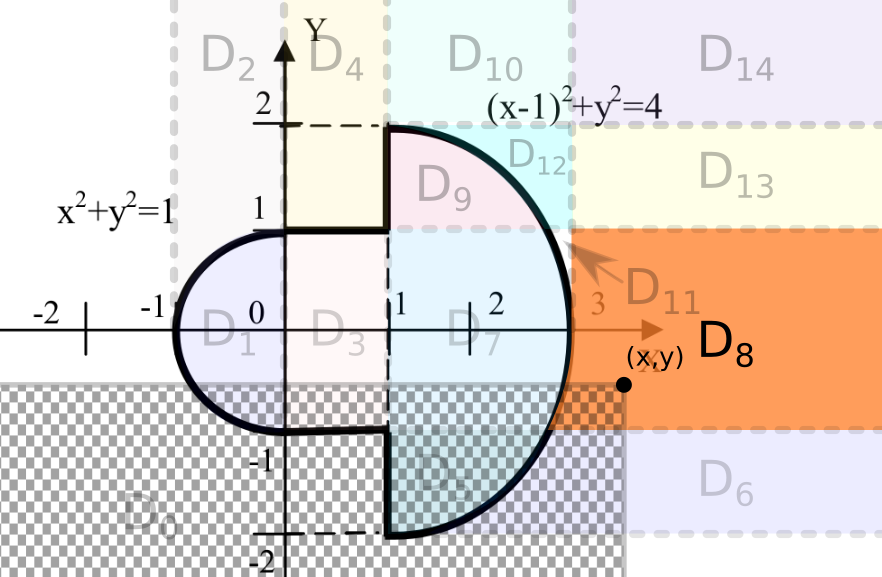
\includegraphics[scale=0.34]{assets/zone945.png} \end{center}
$$
\Fx (x,y) =  \Fx (1+\sqrt{4 - y^2}, y)^{D_7}_{-} =
$$
$$
= \dfrac{\arcsin\left(y\right)+y\sqrt{1-y^2} - \left|  y \right|\sqrt{4-y^2}-4\arcsin\left(\frac{ \left|  y \right|}{2}\right) + 2.5\pi + 2y + 2}{5\pi + 4}
$$

Перевірка:\\
$\frac{\d^2 \Fx}{\d x \d y}(x,y) =
\frac{\d^2}{\d x \d y} \frac{\arcsin\left(y\right)+y\sqrt{1-y^2}+  y  \sqrt{4-y^2}+4\arcsin\left(\frac{y}{2}\right) + 2.5\pi + 2y + 2}{5\pi + 4}  = \frac{\d}{\d y}0 = 0=\fx (x,y)$\\
Далі, знайдемо $\Fx(x,y)^{D_8}$ для $ 0< y < 1$:
$$
\Fx (x,y) =  \Fx (1+\sqrt{4 - y^2}, y)^{D_7}_{+} + \frac{1}{2.5\pi + 2} \cdot  \int\limits_{-y}^{ y}{ds  \int\limits_{1 + \sqrt{4 - y^2}}^{1 + \sqrt{4 -  s^2}}{dt}} =
$$
$$
= \dfrac{\arcsin\left(y\right)+y\sqrt{1-y^2} +  y \sqrt{4-y^2}+4\arcsin\left(\frac{  y }{2}\right) + 2.5\pi + 2y + 2}{5\pi + 4}
$$
Перевірка ліній стику областей:\\
$D_8 - D_7: x = 1 + \sqrt{4 - y^2}$\\
Вже знаходили під час пошуку площі зони:\\
$ \Fx (1 + \sqrt{4 - y^2},y)^{D_7} =  \frac{\arcsin\left(y\right)+y\sqrt{1-y^2}+ \sqrt{4-y^2}+4\arcsin\left(\frac{y}{2}\right) + 2.5\pi + 2y + 2}{5\pi + 4} = \Fx (1 + \sqrt{4 - y^2},y)^{D_8}$\\
$D_8 - D_6: y = -1$\\
$ \Fx (x,-1)^{D_8} = \frac{- \frac{\pi}{2} +0-\sqrt{3}-4\frac{\pi}{6}  + 2.5\pi}{5\pi + 4}
 = \Fx (x,-1)^{D_6}  =  \frac{-\sqrt{3} + 4\frac{-\pi}{2}  + 2\pi }{5\pi +4}$\\
 Повертаємося до зони $D_13:$\\
 $D_8 - D_{13}: y = 1$\\
$
\Fx (x, 1)^{D_8} = \frac{ \frac{\pi}{2} + 0 + \sqrt{3} + 4\frac{\pi }{6} + 2.5\pi + 4  }{5\pi + 4}   = \Fx (x, 1)^{D_13} = \frac{3\pi + 4 + \sqrt{3} + 4\frac{\pi}{6} }{ 5\pi + 4}
$

\newpage



13. $(x,y) \in D_{11}$
\begin{center} 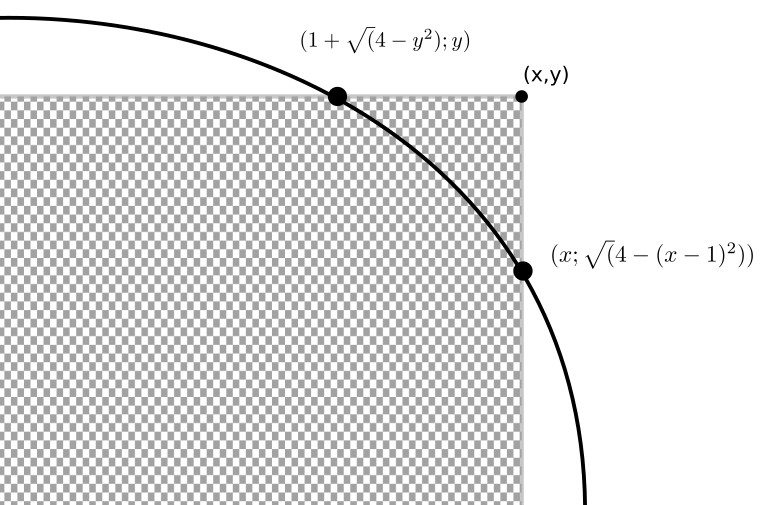
\includegraphics[scale=0.3]{assets/zones13111.png}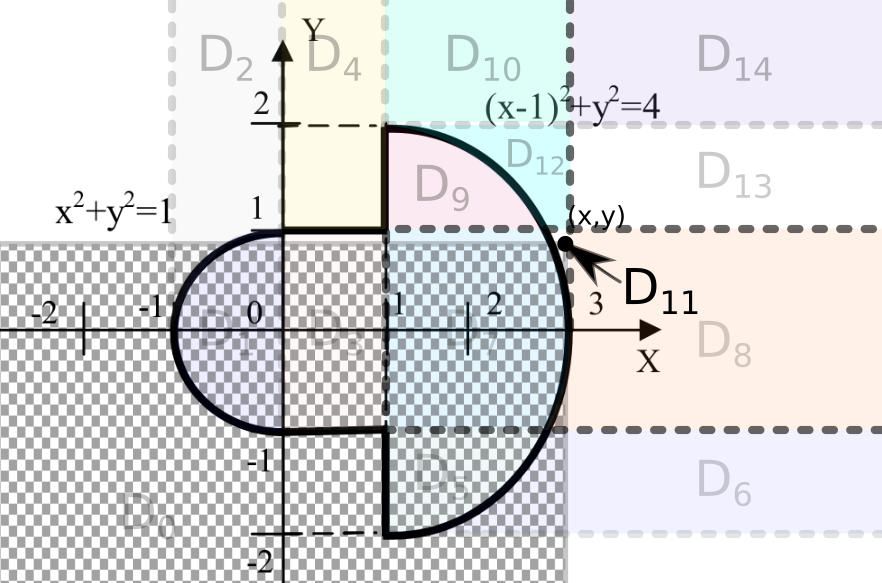
\includegraphics[scale=0.27]{assets/zone13113.png} \end{center}
$$
\Fx (x,y) = \Fx(x,y)^{D_8} -  \frac{1}{2.5\pi + 2} \cdot
 \int\limits_{x}^{3}{ds  \int\limits_{-\sqrt{4 - (s-1)^2}}^{ \sqrt{4 - (s-1)^2}}{dt}} =
$$
$$
 = \frac{\arcsin\left(y\right)+y\sqrt{1-y^2}+  y  \sqrt{4-y^2}+4\arcsin\left(\frac{y}{2}\right) + 2.5\pi + 2y + 2}{5\pi + 4} -
 $$
 $$- \frac{-\left(1-x\right)\sqrt{-x^2+2x+3}-4\arcsin\left(\dfrac{x-1}{2}\right)+2{\pi}}{2.5\pi + 2} =
$$
\begin{center}
$
= \frac{\arcsin\left(y\right)+y\sqrt{1-y^2}+  y  \sqrt{4-y^2}+4\arcsin\left(\frac{y}{2}\right)-  1.5\pi + 2y + 2 +2\left(1-x\right)\sqrt{-x^2+2x+3}+8\arcsin\left(\frac{x-1}{2}\right) }{5\pi + 4}
$
\end{center}


Перевірка:\\
$\frac{\d^2 \Fx}{\d x \d y}(x,y) =
\frac{\d^2}{\d x \d y} \left(  \frac{\arcsin\left(y\right)+y\sqrt{1-y^2}+  y  \sqrt{4-y^2}+4\arcsin\left(\frac{y}{2}\right)-  1.5\pi + 2y + 2 +2\left(1-x\right)\sqrt{-x^2+2x+3}+8\arcsin\left(\frac{x-1}{2}\right) }{5\pi + 4}
\right) =$\\
$ = \dfrac{\d}{ \d y} \left( \frac{-2\sqrt{-x^2+2x+3}-\frac{\left(2-2x\right)\left(x-1\right)}{\sqrt{-x^2+2x+3}}-\frac{4}{\sqrt{1-\frac{\left(x-1\right)^2}{4}}}}{2} \right)  = 0=\fx (x,y)$\\

Перевірка ліній стику областей:\\
$D_{11} - D_6 : x = 3$\\
$ \Fx (3,y)^{D_11} = \frac{\arcsin\left(y\right)+y\sqrt{1-y^2}+  y  \sqrt{4-y^2}+4\arcsin\left(\frac{y}{2}\right) + 2.5\pi + 2y + 2}{5\pi + 4}  = \Fx (x,y)^{D_6}$\\
\newpage

14. $(x,y) \in D_{12}$
\begin{center} 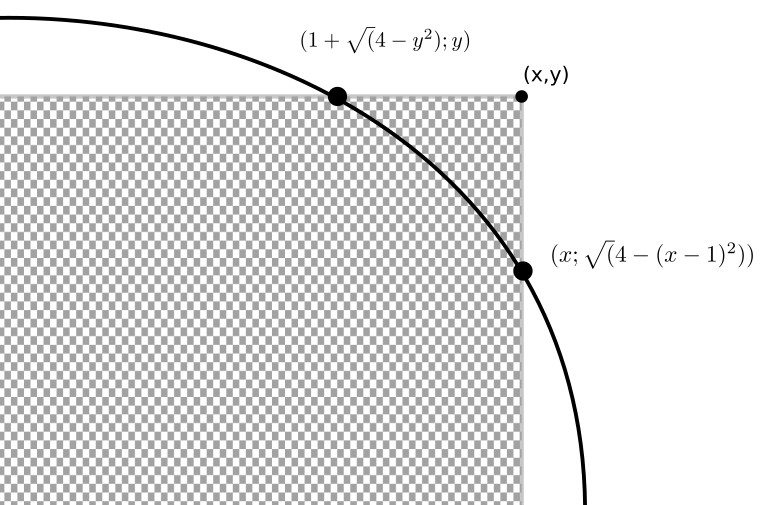
\includegraphics[scale=0.3]{assets/zones13111.png}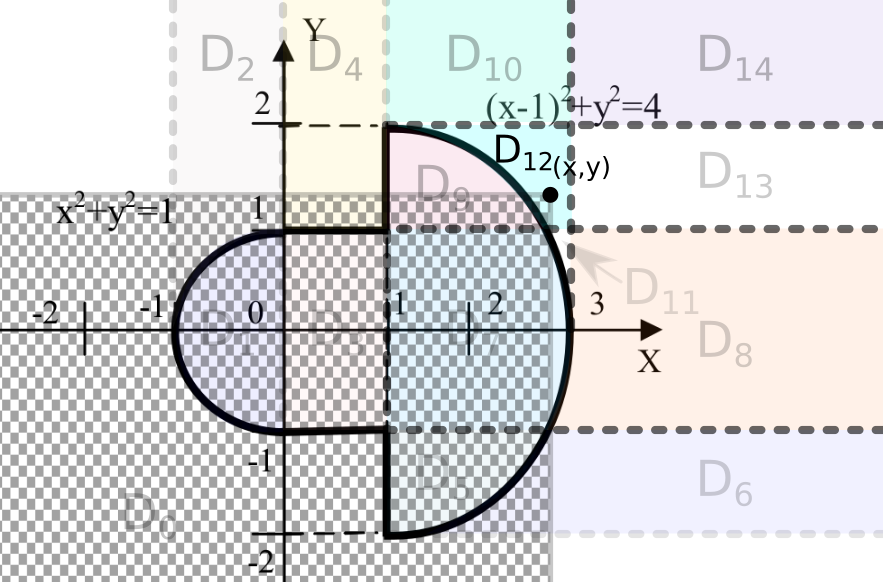
\includegraphics[scale=0.27]{assets/zone14132.png} \end{center}
$$
\Fx (x,y) = \Fx(x,y)^{D_{13}} -  \frac{1}{2.5\pi + 2} \cdot
 \int\limits_{x}^{3}{ds  \int\limits_{-\sqrt{4 - (s-1)^2}}^{ \sqrt{4 - (s-1)^2}}{dt}} =
$$
$$
 = \dfrac{3\pi + 4 + y\sqrt{4-y^2}+4\arcsin\left(\frac{y}{2} \right)}{5\pi + 4} -
 $$
 $$- \frac{-\left(1-x\right)\sqrt{-x^2+2x+3}-4\arcsin\left(\dfrac{x-1}{2}\right)+2{\pi}}{2.5\pi + 2} =
$$
$$
= \frac{ 4-\pi + y\sqrt{4-y^2}+4\arcsin\left(\frac{y}{2} \right) +2\left(1-x\right)\sqrt{-x^2+2x+3}+8\arcsin\left(\frac{x-1}{2}\right) }{5\pi + 4}
$$


Перевірка:\\
$\frac{\d^2 \Fx}{\d x \d y}(x,y) =
\frac{\d^2}{\d x \d y} \left(  \frac{\arcsin\left(y\right)+y\sqrt{1-y^2}+  y  \sqrt{4-y^2}+4\arcsin\left(\frac{y}{2}\right)-  1.5\pi + 2y + 2 +2\left(1-x\right)\sqrt{-x^2+2x+3}+8\arcsin\left(\frac{x-1}{2}\right) }{5\pi + 4}
\right) =$\\
$ = \dfrac{\d}{ \d y} \left( \frac{-2\sqrt{-x^2+2x+3}-\frac{\left(2-2x\right)\left(x-1\right)}{\sqrt{-x^2+2x+3}}-\frac{4}{\sqrt{1-\frac{\left(x-1\right)^2}{4}}}}{2} \right)  = 0=\fx (x,y)$\\

Перевірка ліній стику областей:\\
$D_{12} - D_{13} : x = 3$\\
$ \Fx (3,y)^{D_11} = \dfrac{3\pi + 4 + y\sqrt{4-y^2}+4\arcsin\left(\frac{y}{2} \right)}{5\pi + 4}  = \Fx (x,y)^{D_13}$\\
$D_{12} - D_{13} : y = 2$\\
$ \Fx (x,2)^{D_11} = \frac{ 4-\pi + 0+2\pi +2\left(1-x\right)\sqrt{-x^2+2x+3}+8\arcsin\left(\frac{x-1}{2}\right) }{5\pi + 4} = \frac{ 2+\pi/2 +\left(1-x\right)\sqrt{-x^2+2x+3}+4\arcsin\left(\frac{x-1}{2}\right) }{2.5\pi + 2} = \\= \Fx (x,y)^{D_{10}}$\\

\newpage
15. $(x,y) \in D_{14}$
\begin{center} 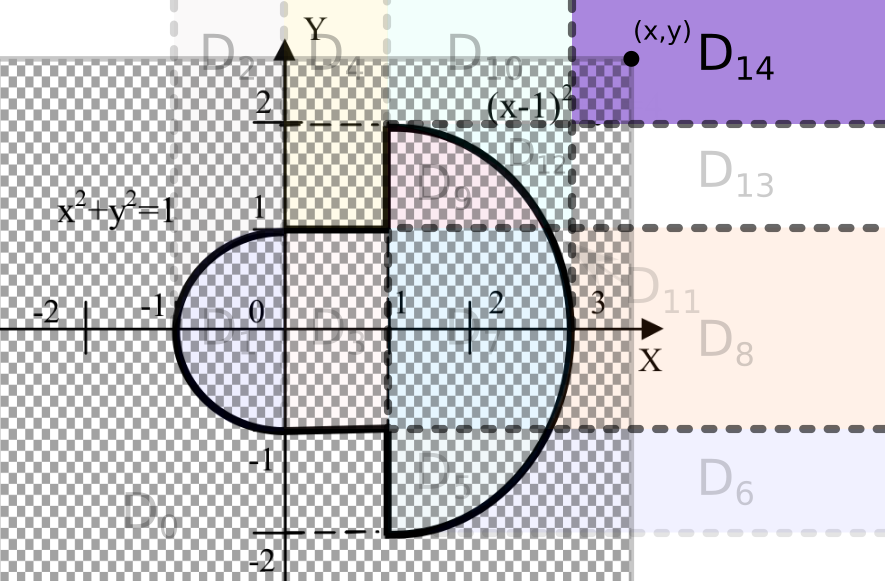
\includegraphics[scale=0.4]{assets/15finalzone.png} \end{center}
$$
\Fx (x,y) = 1
$$
Перевірка:
$\dfrac{\d^2 \Fx}{\d x \d y}(x,y) = 0  = \fx (x,y)$\\
Перевірка ліній стику областей:\\
$D_{14} - D_{10}: x = 3$\\
$ \Fx (3,y)^{D_{10}} = \dfrac{\pi/2+ 2\pi + 2} { 2.5\pi + 2} = 1 =  \Fx (3,y)^{D_{14}} $\\
$D_{14} - D_{13}: y = 1$\\
$ \Fx (x,1)^{D_{13}} = \frac{\pi/2+ 2\pi + 2} { 2.5\pi + 2} = 1 =  \Fx (x,1)^{D_{14}} $\\
$D_{14} - D_{12}: x = 3, y =2$\\
$ \Fx (3,2)^{D_{12}} = \frac{4 - \pi + 2\pi + 4\pi} { 5\pi + 4} = 1 =  \Fx (3,y)^{D_{14}} $\\

\newpage

\epigraph{ Результат выходит далеко за пределы экрана и моего сознания}{Ф. Ницше, 1875 г.}
\textbf{Остаточно отримали відповідь у вигляді системи:}
$$
\Fx(x,y) = \begin{cases}
	0, & (x,y) \in D_{0};\\
	\frac{1}{2.5\pi + 2} \cdot \frac{\arcsin\left(y\right)+y\sqrt{1-y^2}+2xy+\arcsin\left(\sqrt{1-x^2}\right)+3x\sqrt{1-x^2}}{2} , & (x,y) \in D_{1};\\
	 \frac{1}{2.5\pi + 2} \cdot \left( \arcsin\left(\sqrt{1-x^2}\right)+x\sqrt{1-x^2} \right), & (x,y) \in D_{2};\\
	 \frac{1}{2.5\pi + 2} \cdot \left( \frac{\arcsin\left(y\right)+y\sqrt{1-y^2} + \frac{\pi}{2} }{2}+ x(y+1)\right), & (x,y) \in D_{3};\\
	 \frac{1}{2.5\pi + 2} \cdot \left( \frac{\pi}{2}+ 2x\right), & (x,y) \in D_{4};\\
	 \frac{1}{2.5\pi + 2} \cdot \frac{\left(2x-2\right)y+\left(x-1\right)\sqrt{-x^2+2x+3}+4\arcsin\left(\frac{x-1}{2}\right)}{2}, & (x,y) \in D_{5};\\
	 \frac{y\sqrt{4 - y^2} + 4\arcsin\left(\frac{y}{2}\right) + 2\pi }{5\pi +4}, & (x,y) \in D_{6};\\
	 \frac{\arcsin\left(y\right)+y\sqrt{1-y^2} + \frac{\pi}{2} + \left(2-2x\right)+\left(x-1\right)\sqrt{-x^2+2x+3}+4\arcsin\left(\frac{x-1}{2}\right)+ 2x(y+1)}{5\pi + 4},& (x,y) \in D_{7};\\
	 \frac{\arcsin\left(y\right)+y\sqrt{1-y^2} + y\sqrt{4-y^2}+4\arcsin\left(\frac{  y }{2}\right) + 2.5\pi + 2y + 2}{5\pi + 4},& (x,y) \in D_{8};\\
	 \frac{\left(x-1\right)\sqrt{-x^2+2x+3}+4\arcsin\left(\frac{x-1}{2}\right)+4 +2y(x-1) +\pi}{5\pi + 4},& (x,y) \in D_{9};\\
	 \frac{\left(x-1\right)\sqrt{-x^2+2x+3}+4\arcsin\left(\frac{x-1}{2}\right) + \frac{\pi}{2} + 2 }{2.5\pi + 2},& (x,y) \in D_{10};\\
	 \frac{\arcsin\left(y\right)+y\sqrt{1-y^2}+  y  \sqrt{4-y^2}+4\arcsin\left(\frac{y}{2}\right)-  1.5\pi + 2y + 2 }{5\pi + 4}+ \\
	 	 +\frac{2\left(1-x\right)\sqrt{-x^2+2x+3}+8\arcsin\left(\frac{x-1}{2}\right) }{5\pi + 4},& (x,y) \in D_{11};\\
		 \frac{ 4-\pi + y\sqrt{4-y^2}+4\arcsin\left(\frac{y}{2} \right) +2\left(1-x\right)\sqrt{-x^2+2x+3}+8\arcsin\left(\frac{x-1}{2}\right) }{5\pi + 4},& (x,y) \in D_{12};\\
		 \frac{3\pi + 4 + y\sqrt{4-y^2}+4\arcsin\left(\frac{y}{2} \right)}{5\pi + 4},& (x,y) \in D_{13};\\
		 1, & (x,y) \in D_{14};\\
\end{cases}
$$

Нагадаємо маргінальні функції розподілу:

$$
F_{\xi_1} (x) = \begin{dcases}
0, \quad x \leq -1 ;\\
	  \dfrac{\arcsin\left(x\right)+x\sqrt{1-x^2}+\frac{{\pi}}{2} }{2.5\pi + 2} , \quad -1 < x \leq 0; \\
	\dfrac{\frac{{\pi}}{2} +  2x }{2.5\pi + 2} , \quad 0 < x \leq 1; \\
	\dfrac{\left(x-1\right)\sqrt{-x^2+2x+3}+4\arcsin\left(\frac{x-1}{2}\right) + \frac{\pi}{2}+2 }{2.5\pi + 2} , \quad 1 < x \leq 3; \\
	1, \quad x > 3 ;\\
\end{dcases}
$$

$$
F_{\xi_2} (y) = \begin{dcases}
	0, \quad y \leq  -2;\\
 \dfrac{y\sqrt{4-y^2}+4\arcsin\left(\frac{y}{2}\right) + 2{\pi}}{10\pi + 4} , \quad -2 < y \leq -1;\\
 \dfrac{\arcsin\left(y\right)+y\sqrt{1-y^2}+ y\sqrt{4-y^2}+4\arcsin\left(\frac{y}{2}\right) + 2.5\pi + 2y + 2}{5\pi + 4}   ,\\  -1 < y \leq 1; \\
		 	 \dfrac{3\pi + 4 +y\sqrt{4-y^2}+4\arcsin\left(\frac{y}{2}\right)}{5\pi + 4} , \quad 1 < y \leq 2;\\
		1, \quad y >  2;\\
\end{dcases}
$$
Таким чином, за функціє розподілу $\Fx (x,y)$ бачимо, що виконується властивість:
$$
 \lim\limits_{x\to  +\infty}{\Fx (x,y)} = F_{\xi_2}(y) \qquad  \lim\limits_{y\to  \infty}{ \Fx (x,y)} = F_{\xi_1} (x)
$$
$$
\begin{cases}
F_{\xi_1}(x) = 0 = \Fx(x,y)^{D_0}, & x \leq -1 ;\\
F_{\xi_1}(x) = \Fx(x,y)^{D_2}, & -1 < x \leq 0; \\
F_{\xi_1}(x) = \Fx(x,y)^{D_4}, & 0 < x \leq 1; \\
F_{\xi_1}(x) = \Fx(x,y)^{D_{10}}, & 1 < x \leq 3; \\
F_{\xi_1}(x) = \Fx(x,y)^{D_{14}}, & 3 < x; \\
\end{cases}
\quad
\begin{cases}
F_{\xi_2}(y) = 0 = \Fx(x,y)^{D_0}, &y \leq  -2;\\
F_{\xi_2}(y) = \Fx(x,y)^{D_6}, & -2 < y \leq -1;\\
F_{\xi_2}(y) = \Fx(x,y)^{D_8}, & -1 < y \leq 1; \\
F_{\xi_2}(y) = \Fx(x,y)^{D_{13}}, & 1 < y \leq 2;\\
F_{\xi_2}(y) = \Fx(x,y)^{D_{14}}, & y >  2;\\
\end{cases}
$$

\subsection{Математичні
сподівання
координат.
Кореляційна матриця.}

а) Обчислимо математичні сподівання координат.\\
$ \mathbb{E}\xi_1 =  \int\limits_{-\i}^{ +\infty}{ x \cdot f_{\xi_1}(x)dx} = \frac{2}{2.5\pi + 2}\cdot \left( \int\limits_{-1}^{0}{ x\sqrt{(1-x^2)}dx} +  \int\limits_{0}^{ 1}{xdx} +  \int\limits_{1}^{ 3}{x\sqrt{4 - (x-1)^2}dx} \right) =
\\ =
\frac{2}{2.5\pi + 2}\cdot\left( -\frac{\left(1-x^2\right)^\frac{3}{2}}{3} \bigg|_{0}^1  +  \frac{1}{2}  + \frac{8}{3} + \pi  \right) = -\frac{1}{3} +  \frac{1}{2} +  \frac{8}{3} + \pi = \frac{17 + 6 \pi}{3(2.5\pi + 2)} \approx 1.213
$\\
$
\mathbb{E} \xi_2  =  \int\limits_{- \i}^{ +\infty}{ y f_{\xi_2} (y) dy} =\frac{1}{2.5\pi + 2} \cdot \left(  \int\limits_{-2}^{ -1}{  y\sqrt{4 - y^2}dy}  +  \int\limits_{-1}^{ 1}{ y \sqrt{4 - y^2} + y\sqrt{1-y^2}+ y dy}  +\right. $\\$ \left. +   \int\limits_{1}^{ 2}{y \sqrt{4 - y^2}}\right)  =  \int\limits_{-2}^{ 2}{ y\sqrt{4 - y^2}dy} +  \int\limits_{-1}^{ 1}{y\sqrt{1-y^2}+ y dy} = -\frac{\left(4-y^2\right)^\frac{3}{2}}{3}\bigg |_{-2}^{2}+ $\\$+ \left( 	\frac{y^2}{2}-\frac{\left(1-y^2\right)^\frac{3}{2}}{3} \right) \bigg |_{-1}^{1} = 0 + 0 = 0
$ - фігура симетрична відносно $OY$.\\


Окремо розглянемо інтеграли в такому вигляді:
$$
 \int\limits_{}^{ }{t^2 \sqrt{a^2 - (t-b)^2}dt} = \left| \begin{gathered}
s = t-b\\
dt = ds
 \end{gathered} \right|=
$$
$$
=\int\limits_{}^{}{s^2 \sqrt{a^2 - s^2}ds} - 2b  \int\limits_{}^{}{ s \sqrt{a^2 - s^2}ds} + b^2  \int\limits_{}^{}{ \sqrt{a^2 - s^2}ds}
$$
Вже розглядали в загальному вигляді:
$$1. \int\limits_{}^{}{ \sqrt{a^2 - s^2}ds} =  \frac{(t-b) \sqrt{a^2 - (t-b)^2} + a^2 \arcsin{ \frac{(t-b)^2}{a} } }{2} $$
$$
 2.\int\limits_{}^{}{s \sqrt{a^2 - s^2}} = 	\frac{(a^2 - (t-b)^2)^{ \frac{3}{2} 	}} {3}
$$
Знайдемо підстановкою Чєбишева(III):
$$
 \int\limits_{}^{}{ s^2 \sqrt{a^2 -s^2}ds} = \left| \begin{gathered}
  p^2 =  \frac{a^2 - s^2 }{s^2} \\
	\frac{-2a^2}{s^3}ds = 2pdp \\
	sds = \frac{a^2 pdp }{ (p^2 +1)^2}
 \end{gathered} \right|  =  \int\limits_{}^{}{ \frac{a^2p^2}{(p^2 + 1)^2}dp } =
$$
$$
=\frac{\arctan{\left( \sqrt{\frac{a^2 - (t-b)^2}{(t-1)^2}}  \right) }}{2} - \frac{\sqrt{\frac{a^2 - (t-b)^2}{(t-1)^2}}  }{\frac{a^2 - (t-b)^2}{(t-b)^2}+ 2  }
$$
Збираємо разом: \qquad
$
\int\limits_{}^{ }{t^2 \sqrt{a^2 - (t-b)^2}dt} =$\\ \fbox{$=\frac{\arctan{\left( \sqrt{\frac{a^2 - (t-b)^2}{(t-1)^2}}  \right) }}{2} - \frac{\sqrt{\frac{a^2 - (t-b)^2}{(t-1)^2}}  }{\frac{a^2 - (t-b)^2}{(t-b)^2}+ 2  } - 	\frac{(a^2 - (t-b)^2)^{ \frac{3}{2} 	}} {3} + b^2   \frac{(t-b) \sqrt{a^2 - (t-b)^2} + a^2 \arcsin{ \frac{(t-b)^2}{a} } }{2} $}


$\mathbb{E} \xi_1^2  =  \int\limits_{-\i}^{ +\infty}{ x^2  f_{\xi_1} (x)dx} = \frac{2}{2.5\pi + 2}\cdot \left( \int\limits_{-1}^{0}{ x^2\sqrt{(1-x^2)}dx} +  \int\limits_{0}^{ 1}{x^2dx} +  \int\limits_{1}^{ 3}{x^2\sqrt{4 - (x-1)^2}dx} \right) =$\\
$= (*) = \frac{2}{2.5\pi + 2}\cdot \left(\frac{\pi}{16} +  1 + 2 \pi + \frac{16}{3} \right) = \frac{2}{2.5\pi + 2}\cdot \left(2\frac{1}{16}\pi + \frac{19}{3}\right)  \approx  2,1946 $\\
(*) - підстановка чисельних значень в знайдений інтеграл занадто громіздка.\\
$\mathbb{E}\xi_2^2 =   \int\limits_{- \i}^{ +\infty}{ y^2 f_{\xi_2} (y) dy} =\frac{1}{2.5\pi + 2} \cdot \left(  \int\limits_{-2}^{ -1}{  y^2\sqrt{4 - y^2}dy}  +  \int\limits_{-1}^{ 1}{ y^2 \sqrt{4 - y^2} + y^2\sqrt{1-y^2}+ y^2 dy}  +\right. $\\$ \left. +   \int\limits_{1}^{ 2}{y^2 \sqrt{4 - y^2}}\right)  = \frac{1}{2.5\pi + 2} \cdot \left(\frac{8{\pi}+3^\frac{3}{2}}{12} + \frac{19{\pi}-4{\cdot}3^\frac{3}{2}+16}{24} + \frac{8{\pi}+3^\frac{3}{2}}{12} \right) = \frac{51\pi + 16}{12(5\pi +4)} \approx 0,7450 $



Знайдемо дисперсію:\\
$
\mathbb{D}\xi_1 = \mathbb{E}\xi_1^2 - \left( \mathbb{E}\xi_1 \right)^2 = \frac{2}{2.5\pi + 2}\cdot \left(2\frac{1}{16}\pi + \frac{19}{3}\right)  -\frac{144 {{\ensuremath{\pi} }^{2}}+816 \ensuremath{\pi} +1156}{225 {{\ensuremath{\pi} }^{2}}+360 \ensuremath{\pi} +144} = \frac{909 {{\ensuremath{\pi} }^{2}}+2484 \ensuremath{\pi} -976}{900 {{\ensuremath{\pi} }^{2}}+1440 \ensuremath{\pi} +576} \approx 1.1299
$\\
$
\mathbb{D}\xi_2 = \mathbb{E}\xi_2^2 - \left( \mathbb{E}\xi_2 \right)^2 = \frac{51\pi + 16}{12(5\pi +4)} - 0 \approx 0,7451
$
$$
\mathbb{E} \xi_1 \xi_2 =  \int\limits_{-\i}^{+\i}\int\limits_{-\i}^{+\i}{ xy \fx dxdy} =$$
$$=  \frac{1}{2.5\pi + 2}\cdot \left(
 \int\limits_{-1}^{0}{xdx  \int\limits_{\sqrt{1 - x^2}}^{ -\sqrt{1 - x^2}}{ydy}} +
 \int\limits_{0}^{1}{xdx  \int\limits_{\sqrt{1 - x^2}}^{ -\sqrt{1 - x^2}}{ydy}} +  \int\limits_{1}^{3}{xdx  \int\limits_{\sqrt{4 - (x-1)^2}}^{ -\sqrt{4 - (x-1)^2}}{ydy}}
 \right)  =
$$
$$
= \frac{1}{2.5\pi + 2}\cdot \left(
 \int\limits_{-1}^{0}{0 \cdot xdx  } +
 \int\limits_{0}^{1}{0 \cdot xdx  } +  \int\limits_{1}^{3}{0 \cdot xdx  }
 \right)  = 0
$$
Отримали 0, адже фігура симетрична за $OY$.\\
Знайдемо коваріацію та коваріаційну матрицю вектора:
$cov(\xi_1, \xi_2) = \mathbb{E}_{\xi_1, \xi_2} - \mathbb{E}_{\xi_1} \mathbb{E}_{\xi_2} = 0* 0 = 0$

$$
C_{\overline{\xi}} = \begin{bmatrix}
  \dfrac{909 {{\ensuremath{\pi} }^{2}}+2484 \ensuremath{\pi} -976}{900 {{\ensuremath{\pi} }^{2}}+1440 \ensuremath{\pi} +576} & 0\\
	0 &  \dfrac{51\pi + 16}{12(5\pi +4)}
\end{bmatrix} \quad \approx \begin{bmatrix}
  1.1299 & 0\\
 0 &  0,7451
\end{bmatrix}
$$
Очевидно, що матриця додатньовизначена та невироджена.\\
Оскільки коваріація дорівнює 0 $\Rightarrow$ величини $\xi_1, \xi_2$ - некорельовані, слід перевірити координати вектора $\overline{\xi}$ на залежність. Згідно теореми:
\begin{center} 
\includegraphics[scale=0.4]{assets/adf445345.png} \end{center}
Контр-приклад: $0 < x \leq 1$, $-1 < y \leq 1$, в точці (1;1) отримаємо:
$$
 f_{\xi_1}(x) \cdot  f_{\xi_2}(y) = \dfrac{2}{(2.5\pi + 2)^2} \sqrt{(1-x^2)}\cdot  \left( \sqrt{4 - y^2} + \sqrt{1-y^2}+ 1  \right)=
$$
$$
 f_{\xi_1}(1) \cdot  f_{\xi_2}(1) = \dfrac{2}{(2.5\pi + 2)^2} \sqrt{(1-x^2)}\cdot \cdot \left( \sqrt{4 - y^2} + \sqrt{1-y^2}+ 1  \right)= 0 \neq  \dfrac{2}{(2.5\pi + 2)^2}
$$
Тобто, з теореми випливає, що величини залежні.
\newpage

\subsection{Умовні щільності розподілу.}
Нагадаємо:

$$
\fx  (x,y ) = \begin{cases}
	\dfrac{1}{ 2.5\pi + 2}, \quad&(x,y) \in G; \\
	0, \quad& (x,y) \notin G
\end{cases}
$$
$$
f_{\xi_1}(x) = \begin{dcases}
0, \quad x \leq -1 ;\\
 \dfrac{2}{2.5\pi + 2} \sqrt{(1-x^2)}, \quad -1 < x \leq 0; \\
\dfrac{2}{2.5\pi + 2}, \quad 0 < x \leq 1; \\
 \dfrac{2}{2.5\pi + 2} \sqrt{4 - (x-1)^2}, \quad 1 < x \leq 3; \\
	0, \quad x > 3 ;\\
\end{dcases}
$$
$$
f_{\xi_2} (y) = \begin{dcases}
	0, \quad y \leq  -2;\\
	 \dfrac{1}{2.5\pi + 2} \cdot \sqrt{4 - y^2}, \quad -2 < y \leq -1;\\
	\dfrac{1}{2.5\pi + 2} \cdot \left( \sqrt{4 - y^2} + \sqrt{1-y^2}+ 1  \right),  -1 < y \leq 1; \\
	 \dfrac{1}{2.5\pi + 2} \cdot \sqrt{4 - y^2}, \quad 1 < y \leq 2;\\
			0, \quad y >  2;\\
\end{dcases}
$$
\def\undef{\text{ Не визначено }}
Скористаємося формулами:
$$
f_{\xi_{1}} (x | y) = \frac{\fx (x,y)}{f_{\xi_2} (y)} \qquad \quad f_{\xi_{2}} (y | x) = \frac{\fx (x,y)}{f_{\xi_1} (x)}
$$
$$
f_{\xi_1 | \xi_2} (x|y) = \begin{dcases}
\undef, y \leq  -2;\\
\begin{dcases}
		 \dfrac{1}{\sqrt{4 - y^2}}, & -2 < y \leq -1, x \in [1, 1 +\sqrt{4 - y^2}];\\
		 	0, & -2 < y \leq -1, x \notin [1, 1 +\sqrt{4 - y^2}];\\
\end{dcases}\\
\begin{dcases}
\dfrac{1}{\sqrt{4 - y^2} + \sqrt{1-y^2}+ 1}, \quad  -1 < y \leq 1, x \in [-\sqrt{1-y^2}, 1 +\sqrt{4 - y^2}]; \\
0,  -1 < y \leq 1, x \notin [-\sqrt{1-y^2}, \quad 1 +\sqrt{4 - y^2}]; \\
\end{dcases}\\
\begin{dcases}
\dfrac{1}{\sqrt{4 - y^2}} ,&1 < y \leq 2, x \in [1, 1 +\sqrt{4 - y^2}];\\
0 , & 1 < y \leq 2, x \notin [1, 1 +\sqrt{4 - y^2}];\\
\end{dcases}\\
			\undef, y >  2;\\
\end{dcases}
$$
$$
f_{\xi_{2}} (y | x) = \begin{dcases}
\undef, \quad x \leq -1 ;\\
\begin{dcases}
\dfrac{1}{2\sqrt{(1-x^2)}} ,&  -1 < x \leq 0, y \in [-\sqrt{1 - x^2}, \sqrt{1 - x^2}]; \\
 0,&  -1 < x \leq 0, y \notin [-\sqrt{1 - x^2}, \sqrt{1 - x^2}]; \\
\end{dcases}\\
\begin{dcases}
\dfrac{1}{2}, & 0 < x \leq 1, y \in [-1, 1]; \\
0, & 0 < x \leq 1, y \notin [-1, 1]; \\
\end{dcases}\\
\begin{dcases}
\dfrac{1}{2\sqrt{4 - (x-1)^2}}, & 0 < x \leq 1, y \in [-\sqrt{4 - (x-1)^2}, \sqrt{4 - (x-1)^2}]; \\
0, & 0 < x \leq 1, y \notin [-\sqrt{4 - (x-1)^2}, \sqrt{4 - (x-1)^2}]; \\
\end{dcases}\\
	\undef, \quad x > 3 ;\\
\end{dcases}
$$
Перевірка. Очевидними є наступні рівності:\\
$ \int\limits_{1}^{1 +\sqrt{4 - y^2}}{ \dfrac{1}{\sqrt{4 - y^2}dx}} = 1$\\
$ \int\limits_{-\sqrt{1-y^2}}^{1 +\sqrt{4 - y^2}}{ \dfrac{1}{\sqrt{4 - y^2} + \sqrt{1-y^2}+ 1}dx} = 1$\\
$ \int\limits_{-\sqrt{1 - x^2}}^{ \sqrt{1 - x^2}}{\dfrac{1}{2\sqrt{(1-x^2)}} dy} = 1$\\
$ \int\limits_{-1}^{ 1}{\dfrac{1}{2} dy}  = 1$\\
$ \int\limits_{-\sqrt{4 - (x-1)^2}}^{  \sqrt{4 - (x-1)^2}}{\dfrac{1}{2\sqrt{4 - (x-1)^2}}dy} = 1$
Тоді:
\begin{center} 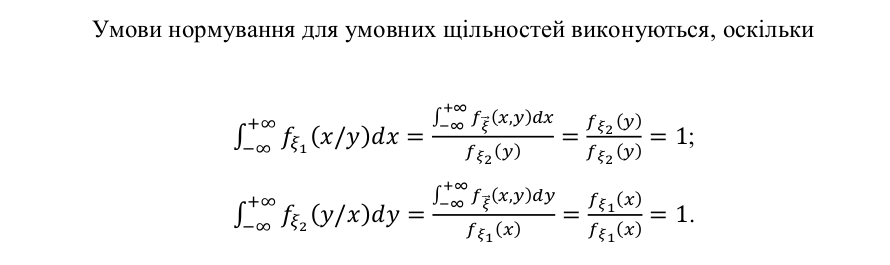
\includegraphics[scale=0.47]{assets/PP_Tereschenko_27_KA96-ae10b36d.png} \end{center}
\newpage

\subsection{Умовні математичні сподівання для кожної координати з
перевіркою.}

$$\mathbb{E}(\xi_1 | \xi_2) =  \int\limits_{-\i}^{ +\infty}{ x\cdot f_{\xi_1 | \xi_2} (x|y) dx}=$$
\vfill

$$
= \begin{dcases}
\undef, y \leq  -2;\\
\int\limits_{-\i}^{ +\infty} x\cdot
\begin{dcases}
		 \dfrac{1}{\sqrt{4 - y^2}}, & -2 < y \leq -1, x \in [1, 1 +\sqrt{4 - y^2}];\\
		 	0, & -2 < y \leq -1, x \notin [1, 1 +\sqrt{4 - y^2}];\\
\end{dcases}\\
\int\limits_{-\i}^{ +\infty} x\cdot
\begin{dcases}
\dfrac{1}{\sqrt{4 - y^2} + \sqrt{1-y^2}+ 1}, \quad  -1 < y \leq 1, x \in [-\sqrt{1-y^2}, 1 +\sqrt{4 - y^2}]; \\
0,  -1 < y \leq 1, x \notin [-\sqrt{1-y^2}, \quad 1 +\sqrt{4 - y^2}]; \\
\end{dcases}\\
\int\limits_{-\i}^{ +\infty} x\cdot
\begin{dcases}
\dfrac{1}{\sqrt{4 - y^2}} ,&1 < y \leq 2, x \in [1, 1 +\sqrt{4 - y^2}];\\
0 , & 1 < y \leq 2, x \notin [1, 1 +\sqrt{4 - y^2}];\\
\end{dcases}\\
			\undef, y >  2;\\
\end{dcases} =
$$
\vfill

$$
= \begin{dcases}
\undef, y \leq  -2;\\
\int\limits_{1}^{ 1 +\sqrt{4 - y^2}} x\cdot
		 \dfrac{1}{\sqrt{4 - y^2}}dx, \quad -2 < y \leq -1;\\
\int\limits_{-\sqrt{1-y^2}}^{ 1 +\sqrt{4 - y^2}} x\cdot
\dfrac{1}{\sqrt{4 - y^2} + \sqrt{1-y^2}+ 1}dx, \quad  -1 < y \leq 1; \\
\int\limits_{1}^{ 1 +\sqrt{4 - y^2}} x\cdot
\dfrac{1}{\sqrt{4 - y^2}} ,1 < y \leq 2;\\
			\undef, y >  2;\\
\end{dcases} =
$$
\vfill
\newpage
$$
= \begin{dcases}
\undef, y \leq  -2;\\
\dfrac{x^2}{2\sqrt{4-y^2}} \Bigg|_{1}^{ 1 +\sqrt{4 - y^2}},              \quad -2 < y \leq -1;\\
\dfrac{x^2}{2\left(\sqrt{4-y^2}+\sqrt{1-y^2}+1\right)}\Bigg|_{-\sqrt{1-y^2}}^{ 1 +\sqrt{4 - y^2}} ,             \quad  -1 < y \leq 1; \\
\dfrac{x^2}{2\sqrt{4-y^2}} \Bigg|_{1}^{ 1 +\sqrt{4 - y^2}},               \quad 1 < y \leq 2;\\
			\undef, y >  2;\\
\end{dcases} =
$$

$$
= \begin{dcases}
\undef, y \leq  -2;\\
\dfrac{\sqrt{4-y^2}+2}{2},              \quad -2 < y \leq -1;\\
\dfrac{\sqrt{4-y^2}-\sqrt{1-y^2}+1}{2},             \quad  -1 < y \leq 1; \\
\dfrac{\sqrt{4-y^2}+2}{2},               \quad 1 < y \leq 2;\\
			\undef, y >  2;\\
\end{dcases}
$$
Перевірка:
$$
\mathbb{E} \left( \mathbb{E}(\xi_1 | \xi_2) \right)  =  \int\limits_{-\i}^{ +\infty}{\mathbb{E}(\xi_1 | \xi_2)} f_{\xi_2}dy =  \int\limits_{-2}^{ -1}{
 \dfrac{1}{2.5\pi + 2} \cdot \sqrt{4 - y^2}\dfrac{\sqrt{4-y^2}+2}{2}dy} +
$$
$$
+  \int\limits_{-1}^{ 1}{\dfrac{1}{2.5\pi + 2} \cdot \left( \sqrt{4 - y^2} + \sqrt{1-y^2}+ 1  \right) \dfrac{\sqrt{4-y^2}-\sqrt{1-y^2}+1}{2} dy}+
$$
$$
+\int\limits_{1}^{ 2}{
 \dfrac{1}{2.5\pi + 2} \cdot \sqrt{4 - y^2}\dfrac{\sqrt{4-y^2}+2}{2}dy}=
$$
$$
= \int\limits_{-2}^{ -1}{
\dfrac{2\sqrt{4-y^2}+4 - y^2}{5\pi + 4}dy} + \int\limits_{-1}^{ 1}{
\dfrac{2\sqrt{4-y^2}+4 }{5\pi + 4}dy} +  \int\limits_{1}^{ 2}{
\dfrac{2\sqrt{4-y^2}+4 - y^2}{5\pi + 4}dy} =
$$
$$
= 2 \cdot \dfrac{4{\pi}-3^\frac{3}{2}+5}{15{\pi}+12}+
\dfrac{4{\pi}+2{\cdot}3^\frac{3}{2}+24}{3\left(5{\pi}+4\right)} = \frac{12\pi + 34 }{3\left(5{\pi}+4\right)}  = \frac{3\pi + 17}{3\left(2.5{\pi}+2\right)}  = \mathbb{E} \xi_1
$$
\newpage
\vfill

$$\mathbb{E}(\xi_2 | \xi_1) =  \int\limits_{-\i}^{ +\infty}{ y\cdot f_{\xi_2 | \xi_1} (y|x) dy}=$$
\vfill

$$
= \begin{dcases}
\undef, \quad x \leq -1 ;\\
\int\limits_{-\i}^{ +\i} y \cdot
\begin{dcases}
 \dfrac{1}{2\sqrt{(1-x^2)}} ,  -1 < x \leq 0, y \in [-\sqrt{1 - x^2}, \sqrt{1 - x^2}]; \\
 0,  -1 < x \leq 0, y \notin [-\sqrt{1 - x^2}, \sqrt{1 - x^2}]; \\
\end{dcases}\\
 \int\limits_{-\i}^{ +\i} y \cdot \begin{dcases}
\dfrac{1}{2},  0 < x \leq 1, y \in [-1, 1]; \\
0,   < x \leq 1, y \notin [-1, 1]; \\
\end{dcases}\\
 \int\limits_{-\i}^{ +\i} y \cdot \begin{dcases}
\dfrac{1}{2\sqrt{4 - (x-1)^2}},  0 < x \leq 1, y \in [-\sqrt{4 - (x-1)^2}, \sqrt{4 - (x-1)^2}]; \\
0,  0 < x \leq 1, y \notin [-\sqrt{4 - (x-1)^2}, \sqrt{4 - (x-1)^2}]; \\
\end{dcases}\\
	\undef, \quad x > 3 ;\\
\end{dcases} =
$$
\vfill

$$
=\begin{dcases}
\undef, \quad x \leq -1 ;\\
\int\limits_{-\sqrt{1 - x^2}}^{ \sqrt{1 - x^2}} y \cdot
 \dfrac{1}{2\sqrt{(1-x^2)}} , \quad -1 < x \leq 0; \\
 \int\limits_{-1}^{ +1} y \cdot
\dfrac{1}{2}, \quad 0 < x \leq 1; \\
 \int\limits_{-\sqrt{4 - (x-1)^2}}^{\sqrt{4 - (x-1)^2}} y \cdot
\dfrac{1}{2\sqrt{4 - (x-1)^2}},\quad  1 < x \leq 3; \\
	\undef, \quad x > 3 ;\\
\end{dcases} =
$$
\vfill
$$
=\begin{dcases}
\undef, \quad x \leq -1 ;\\
\dfrac{y^2}{4\sqrt{1-x^2}}\Bigg|_{-\sqrt{1 - x^2}}^{ \sqrt{1 - x^2}} , \quad -1 < x \leq 0; \\
 \dfrac{y^2}{4}\Bigg|_{-1}^{ +1}
, \quad 0 < x \leq 1; \\
\dfrac{y^2}{4\sqrt{4 - (x-1)^2}} \Bigg|_{-\sqrt{4 - (x-1)^2}}^{\sqrt{4 - (x-1)^2}}
,\quad 1 < x \leq 3; \\
	\undef, \quad x > 3 ;\\
\end{dcases} =
\fbox{$\begin{dcases}
\undef, \quad x \leq -1 ;\\
0,\quad -1 < x \leq 3; \\
	\undef, \quad x > 3 ;\\
\end{dcases}$}
$$
Перевірка:
$$
\mathbb{E} \left( \mathbb{E}(\xi_2 | \xi_1) \right)  =  \int\limits_{-\i}^{ +\infty}{\mathbb{E}(\xi_2| \xi_1)} f_{\xi_1}dy =  \int\limits_{-\i}^{ +\infty}{0 \cdot f_{\xi_1}dy} =  0 = \mathbb{E}\xi_2
$$
\newcommand{\heart}{\ensuremath\heartsuit}
\begin{center}
	\Large \heart
\end{center}
\end{document}
